% !TeX program = pdflatex
% !TeX spellcheck = en_US
% !TeX encoding = UTF-8

% update
% v1.13 - 2020-01-15
% - Tanja: change the style.tex: define Black as a color and use it to replace DarkRed (except on the title page)
% - Tanja: change the the titlepage once more 
% - Tanja: change the color code for DarkRed to match the current TU logo sytle
% v1.12 - 2020-01-02
% - Tanja: add new titlepage design and replace all logos with the new one
% v1.11 - 2018-10-15
% - Felix: use Bibtex instead of Biblatex
% v1.10 - 2017-05-30
% - Erik: Refactor the file structure of the front pages
% - Erik: Fix double bibliography entry
% v1.9 - 2017-02-03
% - Dirk: fixed warning: Underfull \hbox (badness 10000) in paragraph main.tex
% - Dirk: fixed warning: "Data encoding is UTF8" -> style.tex 0.1.8
% v1.8 - 2017-02-02
% - Dirk: replaced titlesec package by KOMA-script commands.-> style.tex v0.1.7
% v1.7 - 2014-11-18
% - bib fixes: now using biber instead of bibtex (thanks felix)
% - compile now with pdflatex -> biber -> pdflatex
% v1.6 - 2013-05-13
% - bibliography headers fixed - thanx lorenz lehmann
% - high quality titlepage - thanx thomas graf
% - removed separation of online and offline references -> style 1.4a
% v1.5 - 2013-01-16

\documentclass[twoside,11pt,titlepage,a4paper,english,bibliography=totocnumbered,listof=numbered]{scrbook}
%
% Template Style
% =========================================================================
% = SNET THESIS TEMPLATE STYLE
% =========================================================================

% http://www.snet.tu-berlin.de
% ------------------------
% Adapted version from http://hci.rwth-aachen.de/karrer_thesistemplate (Thorsten Karrer)
% Further adaptions for http://www.elearn.rwth-aachen.de (Sascha Hoellger)
% Further adaptions for SNET @ TU Berlin by Sebastian Göndör (sebastian.goendoer@tu-berlin.de)


% =========================================================================
% = CHANGELOG
% =========================================================================
% [0.1.9]
% - Fixed styling for chapters and toc using Komascript
% - Remove double bibliography TOC entry
%
% [0.1.8]
% - fixed "warning UFT8 is used". biblatex requires ascii encoding; by Dirk
%
% [0.1.7]
% replaced "Titelsec" commands (and whole package) by appropriate KOMA-Script commands; by Dirk
%
% [0.1.6]
% replaced deprecated \rm commands with \rmfamily commands; by Dirk
%
% [0.1.4b]
% backend=biber added in line 139
%
% [0.1.4a]
% title page: image logo sizes and margins adjusted to printable area
% removed separation of online and offline references
%
% [0.1.3]
% wider text body
% added "school" to the titlepage
% paragraph indents
% correctly placed footnote graphics
%
% [0.1.2]
% new titlepage
% some minor fixes
%
% [0.1.1]
% changed titlepage logo
% added listoffigures and listoftables
% excluded abstract from toc
% no (roman) numbering for frontmatter
%
% [0.1]
% adapted version 0.991b from sascha hoellger @ rwth aachen


% =========================================================================
% = MISC
% =========================================================================

\usepackage{a4wide}					%
\usepackage{verbatim}				%
\usepackage[toc,page]{appendix}			%
\usepackage[withpage]{acronym}			%
\usepackage{amsthm}				% Definitions


% =========================================================================
% = COLORS
% =========================================================================

\usepackage{xcolor}					% Colors
\definecolor{codeback}{rgb}{.8,.8,.8,}
\definecolor{LightBlue}{rgb}{0.55,0.55,1}
\definecolor{DarkBlue}{rgb}{0.2,0.2,0.5}
\definecolor{DarkRed}{rgb}{0.7725490196,0.05490196078,0.12549019607} % new TU red
\definecolor{Black}{rgb}{0,0,0}

% =========================================================================
% = Listing style (code)
% =========================================================================

% =========================================================================
% = PAGE LAYOUT
% =========================================================================

\usepackage{geometry}
\geometry{inner=3cm, outer=2cm, bottom=4cm}

\newcommand{\setwidesite}				% changes the geometry to have less margin
{
	\fancyhfoffset[LE,RO]{0cm}
	\fancyheadoffset[LO,RE]{0cm}
	\fancyfootoffset[RE]{2cm}
	\newgeometry{inner=2cm, outer=2cm, bottom=4cm}
}

\usepackage{style/noindent}				%do not indent at new paragraphs but add a vertical offset

\setlength{\parindent}{4mm}
\setlength{\parskip}{1.5mm }


% =========================================================================
% = TYPESETTING
% =========================================================================

\usepackage[hyphens]{url}				% url
\usepackage{hyphenat}				% hyphenation. use \hyphenation{}

\righthyphenmin=5
\lefthyphenmin=5


% =========================================================================
% = TABLE OF CONTENTS
% =========================================================================

\setcounter{secnumdepth}{4}
\setcounter{tocdepth}{3}

\addtokomafont{disposition}{\rmfamily}


% =========================================================================
% = FONTS
% =========================================================================

\usepackage{mathpazo}
\usepackage[scaled=.95]{helvet}
\usepackage{courier}


% =========================================================================
% = SYMBOLS
% =========================================================================

%\usepackage{gensymb}
\usepackage{textcomp} 				% for \textmu (non-italic $\mu$)
\makeatletter						% this makes "@" a regular letter


% =========================================================================
% = TABLES
% =========================================================================

\usepackage{tabularx}
\usepackage{booktabs}
\usepackage{multirow}
\usepackage{longtable}				% tables spanning over more than one page

%%\setlength{\fboxsep}{0mm}			% spacing between \fbox border and content

\usepackage{amsmath}				% math fonts
\usepackage{amssymb}				% math symbols
\usepackage{setspace}				% line spacing


% =========================================================================
% = BIBILOGRAPHY
% =========================================================================

% 2018-10-16 - changed to use Bibtex instead

%\usepackage[style=numeric,natbib=true,backend=biber]{biblatex}

% apparently no effect?
%\renewcommand{\bibsetup}{
%	\markboth{
%		\MakeUppercase{Bibliography}
%	}{}
%}

%\ifdefined\bibheadingonline
%  \defbibheading{online}{\section*{\bibheadingonline}}
%\else
%  \defbibheading{online}{\section*{Online References}}
%\fi
%\ifdefined\bibheadingoffline
%  \defbibheading{offline}{\section*{\bibheadingoffline}}
%\else
%  \defbibheading{offline}{\section*{Printed References}}
%\fi
%
%\defbibfilter{online}{%
%  \( \type{online} \)}
%
%\defbibfilter{offline}{%
%  \( \not \type{online} \)}
%
%\bibliography{Bibliography}


% =========================================================================
% = LANGUAGE & ENCODING
% =========================================================================

\usepackage[english]{babel}				% \usepackage[ngerman]{babel}

\selectlanguage{english}				% \selectlanguage{ngerman}

\usepackage[T1]{fontenc}
\usepackage[utf8]{inputenc}				% can use native umlauts

% \usepackage[babel,german=quotes]{csquotes}	% provides \enquote{Blupp} => "`Blupp"'
\usepackage[babel,english=american]{csquotes}	% provides \enquote{Blupp} => "`Blupp"'

%\SetCiteCommand{\parencite}			% Changed for biblatex

\usepackage{units}					% unified way of setting values with units

\usepackage{appendix}


% =========================================================================
% = CODE LISTINGS
% =========================================================================

\usepackage{listings}

% Listings Styles from Max

\definecolor{violet}{cmyk}{0.45,0.97,0.27,0.21}
\definecolor{lstblue}{cmyk}{1,0.80,0,0}
\definecolor{lstgreen}{cmyk}{0.71,0.21,0.65,0.22}
\definecolor{bluegrey}{cmyk}{0.56,0.24,0.11,0.05}
\definecolor{javadoc}{cmyk}{0.88,0.59,0,0}
\definecolor{lstgrey}{cmyk}{0.55,0.44,0.42,0.32}

\lstdefinelanguage{SQL}{
     keywords={},
     keywordstyle=\color{bluegrey}\bfseries,
     morekeywords=[2]{CREATE,TABLE,IF,NOT,EXISTS,NULL,SET,DEFAULT,PRIMARY,KEY,COLLATE,CHARACTER,AUTO_INCREMENT,ENGINE,CHARSET},
     keywordstyle={[2]\color{violet}\bfseries},
     otherkeywords={int,varchar,double,text,tinyint},
     sensitive=false,
     morecomment=[l][\color{lstgreen}]{//},
     morecomment=[s][\color{lstgreen}]{/*}{*/},
     morecomment=[s][\color{javadoc}]{/**}{*/},
     morestring=[b]',
     morestring=[b]"
  }
\lstdefinelanguage{PHP}{
     keywords={},
     keywordstyle=\color{bluegrey}\bfseries,
     morekeywords=[2]{static,function,if,return,pow,sin,cos,asin,min,sqrt,int},
     keywordstyle={[2]\color{violet}\bfseries},
     otherkeywords={@param, @returns, @author, @type, @link, @see},
     sensitive=false,
     morecomment=[l][\color{lstgreen}]{//},
     morecomment=[s][\color{lstgreen}]{/*}{*/},
     morecomment=[s][\color{javadoc}]{/**}{*/},
     morestring=[b]',
     morestring=[b]"
  }

% \lstdefinelanguage{JavaScript}{
%      keywords={},
%      keywordstyle=\color{bluegrey}\bfseries,
%      morekeywords=[2]{attributes, class, classend, do, empty, endif, endwhile, fail, function, functionend, if, implements, in, inherit, inout, not, of, operations, out, return, set, then, types, while, use},
%      keywordstyle={[2]\color{violet}\bfseries},
%      otherkeywords={@param, @returns, @author, @type, @link, @see},
%      sensitive=false,
%      morecomment=[l][\color{lstgreen}]{//},
%      morecomment=[s][\color{lstgreen}]{/*}{*/},
%      morecomment=[s][\color{javadoc}]{/**}{*/},
%      morestring=[b]',
%      morestring=[b]"
%   }

\lstdefinelanguage{JavaScript}{
  keywords={abstract, any, as, boolean, break, case, catch, class, console, 
      const, continue, debugger, declare, default, delete, do, else, enum, export, 
      extends, false, finally, for, from, function, get, if, implements, import, in, 
      infer, instanceof, interface, keyof, let, module, namespace, never, new, null, 
      number, package, private, protected, public, readonly, require, return, 
      set, static, string, super, switch, symbol, this, throw, true, try, type, typeof, 
      undefined, unique, unknown, var, void, while, with, yield}
  keywordstyle=\color{blue}\bfseries,
  ndkeywords={class, export, boolean, throw, implements, import, this},
  ndkeywordstyle=\color{darkgray}\bfseries,
  identifierstyle=\color{black},
  sensitive=false,
  comment=[l]{//},
  morecomment=[s]{/*}{*/},
  commentstyle=\color{purple}\ttfamily,
  stringstyle=\color{red}\ttfamily,
  morestring=[b]',
  morestring=[b]"
}

\lstset{
   language=JavaScript,
   extendedchars=true,
   basicstyle=\footnotesize\ttfamily,
   showstringspaces=false,
   showspaces=false,
   numbers=left,
   numberstyle=\footnotesize,
   numbersep=9pt,
   tabsize=2,
   breaklines=true,
   showtabs=false,
   captionpos=b
}

\lstdefinelanguage{Java}{
     keywords={},
     keywordstyle=\color{bluegrey}\bfseries,
     morekeywords=[2]{abstract,boolean,break,byte,case,catch,char,class,
      const,continue,default,do,double,else,extends,false,final,
      finally,float,for,goto,if,implements,import,instanceof,int,
      interface,label,long,native,new,null,package,private,protected,
      public,return,short,static,super,switch,synchronized,this,throw,
      throws,transient,true,try,void,volatile,while},
     keywordstyle={[2]\color{violet}\bfseries},
     morekeywords=[3]{@SuppressWarnings, @Capability, @Override},
     keywordstyle={[3]\color{lstgrey}},
     otherkeywords={@param, @return, @returns, @author, @link, @see},
     sensitive,
     morecomment=[l]//,
     morecomment=[s]{/*}{*/},
     morecomment=[s][\color{javadoc}]{/**}{*/},
     morestring=[b]",
     morestring=[b]',
  }[keywords,comments,strings]

% some listings styles from Gregor Aisch
% http://vis4.net/blog/2009/09/noch-mehr-sprach-definitionen-fuer-latex-listings/

\lstdefinelanguage{HTML5} {morekeywords={a, abbr, address, area, article, aside, audio, b, base, bb, bdo, blockquote,  body, br, button, canvas, caption, cite, code, col, colgroup, command, datagrid, datalist, dd, del, details, dialog, dfn, div, dl, dt, em, embed, eventsource, fieldset, figure, footer,  form,  h1, h2,  h3,  h4, h5,  h6,  head,  header,  hr, html,  i, iframe,  img,  input,  ins, kbd,  label,  legend,  li,  link,  mark,  map,  menu,  meta,  meter,  nav,  noscript,  object,  ol,  optgroup,  option,  output,  p,  param,  pre,  progress,  q,  ruby,  rp,  rt,  samp,  script,  section,  select,  small,  source,  span,  strong,  style,  sub,  sup,  table,  tbody,  td,  textarea,  tfoot,  th,  thead,  time,  title,  tr,  ul,  var,  video},
sensitive=false, morecomment=[s]{<!--}{-->}, morestring=[b]", morestring=[d]'}

\lstdefinelanguage{CSS} {morekeywords={azimuth,  background-attachment,  background-color,  background-image,  background-position,  background-repeat,  background,  border-collapse,  border-color,  border-spacing,  border-style,  border-top, border-right, border-bottom, border-left,  border-top-color, border-right-color, border-bottom-color, border-left-color,  border-top-style, border-right-style, border-bottom-style, border-left-style,  border-top-width, border-right-width, border-bottom-width, border-left-width,  border-width,  border,  bottom,  caption-side,  clear,  clip,  color,  content,  counter-increment,  counter-reset,  cue-after,  cue-before,  cue,  cursor,  direction,  display,  elevation,  empty-cells,  float,  font-family,  font-size,  font-style,  font-variant,  font-weight,  font,  height,  left,  letter-spacing,  line-height,  list-style-image,  list-style-position,  list-style-type,  list-style,  margin-right, margin-left,  margin-top, margin-bottom,  margin,  max-height,  max-width,  min-height,  min-width,  orphans,  outline-color,  outline-style,  outline-width,  outline,  overflow,  padding-top, padding-right, padding-bottom, padding-left,  padding,  page-break-after,  page-break-before,  page-break-inside,  pause-after,  pause-before,  pause,  pitch-range,  pitch,  play-during,  position,  quotes,  richness,  right,  speak-header,  speak-numeral,  speak-punctuation,  speak,  speech-rate,  stress,  table-layout,  text-align,  text-decoration,  text-indent,  text-transform,  top,  unicode-bidi,  vertical-align,  visibility,  voice-family,  volume,  white-space,  widows,  width,  word-spacing,  z-index},
sensitive=false, morecomment=[s]{/*}{*/}, morestring=[b]", morestring=[d]'}

\lstdefinelanguage{JavaFX} {morekeywords={abstract, after, and, as, assert, at, attribute, before, bind, bound, break, catch, class, continue, def, delete, else, exclusive, extends, false, finally, first, for, from, function, if, import, indexof, in, init, insert, instanceof, into, inverse, last, lazy, mixin, mod, new, not, null, on, or, override, package, postinit, private, protected, public-init, public, public-read, replace, return, reverse, sizeof, static, step, super, then, this, throw, trigger, true, try, tween, typeof, var, where, while, with },
sensitive=false, morecomment=[l]{//}, morecomment=[s]{/*}{*/}, morestring=[b]", morestring=[d]'}

\lstdefinelanguage{MXML} {morekeywords={mx:Accordion, mx:Box, mx:Canvas, mx:ControlBar, mx:DividedBox, mx:Form, mx:FormHeading, mx:FormItem, mx:Grid, mx:GridItem, mx:GridRow, mx:HBox, mx:HDividedBox, mx:LinkBar, mx:Panel, mx:TabBar, mx:TabNavigator, mx:Tile, mx:TitleWindow, mx:VBox, mx:VDividedBox, mx:ViewStack, mx:Button, mx:CheckBox, mx:ComboBase, mx:ComboBox, mx:DataGrid, mx:DateChooser, mx:DateField, mx:HRule, mx:Image, mx:Label, mx:Link, mx:List, mx:Loader, mx:MediaController, mx:MediaDisplay, mx:MediaPlayback, mx:MenuBar, mx:NumericStepper, mx:ProgressBar, mx:RadioButton, mx:RadioButtonGroup, mx:Spacer, mx:Text, mx:TextArea, mx:TextInput, mx:Tree, mx:VRule, mx:VScrollBar, mx:Application, mx:Repeater, mx:UIComponent, mx:UIObject, mx:View, mx:FlexExtension, mx:UIComponentExtension, mx:UIObjectExtension, mx:Fade, mx:Move, mx:Parallel, mx:Pause, mx:Resize, mx:Sequence, mx:WipeDown, mx:WipeLeft, mx:WipeRight, mx:WipeUp, mx:Zoom, mx:EventDispatcher, mx:LowLevelEvents, mx:UIEventDispatcher, mx:CurrencyFormatter, mx:DateFormatter, mx:NumberFormatter, mx:PhoneFormatter, mx:ZipCodeFormatter, mx:CursorManager, mx:DepthManager, mx:DragManager, mx:FocusManager, mx:HistoryManager, mx:LayoutManager, mx:OverlappedWindows, mx:PopUpManager, mx:SystemManager, mx:TooltipManager, mx:CreditCardValidator, mx:DateValidator, mx:EmailValidator, mx:NumberValidator, mx:PhoneNumberValidator, mx:SocialSecurityValidator, mx:StringValidator, mx:ZipCodeValidator, mx:DownloadProgressBar, mx:ArrayUtil, mx:ClassUtil, mx:Delegate, mx:ObjectCopy, mx:URLUtil, mx:XMLUtil, mx:CSSSetStyle, mx:CSSStyleDeclaration, mx:CSSTextStyles, mx:StyleManager, mx:HTTPService, mx:RemoteObject, mx:Service},
sensitive=false, morecomment=[s]{<!--}{-->}, morestring=[b]", morestring=[d]'}

\lstdefinelanguage{LZX} {morekeywords={a, alert, animator, animatorgroup , attribute, audio , axis, axisstyle , b, barchart, basebutton , basebuttonrepeater , basecombobox , basecomponent , basedatacombobox , basedatepicker , basedatepickerday , basedatepickerweek , basefloatinglist , basefocusview , baseform , baseformitem , basegrid , basegridcolumn , baselist , baselistitem , basescrollarrow , basescrollbar , basescrollthumb , basescrolltrack , baseslider , basestyle , basetab , basetabelement , basetabpane , basetabs , basetabsbar , basetabscontent , basetabslider , basetrackgroup , basetree , basevaluecomponent , basewindow , br , button , canvas , chart , chartbgstyle , chartstyle , checkbox , class , columnchart , combobox , command , connection , connectiondatasource , constantboundslayout , constantlayout , datacolumn , datacombobox , datalabel , datamarker , datapath , datapointer , dataselectionmanager , dataseries , dataset , datasource , datastyle , datastylelist , datatip , datepicker , debug , dragstate , drawview , edittext , event , face , floatinglist , font , font , form , frame , grid , gridcolumn , gridtext , handler , hbox , horizontalaxis , hscrollbar , i , image , img , import , include , inputtext , javarpc , label , labelstyle , layout , legend , library , linechart , linestyle , list , listitem , LzTextFormat , menu , menubar , menuitem , menuseparator , method , modaldialog , multistatebutton , node , p , param , piechart , piechartplotarea , plainfloatinglist , plotstyle , pointstyle , pre , radiobutton , radiogroup , rectangularchart , regionstyle , remotecall , resizelayout , resizestate , resource , reverselayout , richinputtext , rpc , script , scrollbar , security , selectionmanager , sessionrpc , simpleboundslayout , simpleinputtext , simplelayout , slider , soap , splash , stableborderlayout , state , statictext , style , submit , swatchview , SyncTester , tab , tabelement , tabpane , tabs , tabsbar , tabscontent , tabslider , Test , TestCase , TestResult , TestSuite , text , textlistitem , tickstyle , tree , u , valueline , valuelinestyle , valuepoints , valuepointstyle , valueregion , valueregionstyle , vbox , verticalaxis , view , view , vscrollbar , webapprpc , window , windowpanel , wrappinglayout , XMLHttpRequest , xmlrpc , zoomarea},
sensitive=false, morecomment=[s]{<!--}{-->}, morestring=[b]", morestring=[d]'}

\lstset{
  numbers=left,
  numberstyle=\tiny,
  numbersep=5pt,
  breaklines=true,
  stepnumber=1,
  tabsize=2,
  basicstyle=\ttfamily\small,
  frame=single,
  numberfirstline=true,
  firstnumber=1,
  keywordstyle=\color{violet}\bfseries,
  ndkeywordstyle=\color{bluegrey}\bfseries,
  identifierstyle=\color{black},
  commentstyle=\color{lstgreen}\ttfamily,
  stringstyle=\color{lstblue}\ttfamily,
  showstringspaces=false
    backgroundcolor=\color{gray!10!white},
}


% ========================================================================
% = CHANGE LIST DEFINITIONS
% ========================================================================

% change color of item list
\renewcommand{\labelitemi}{\color{Black}$\bullet$}
\renewcommand{\labelitemii}{\color{Black}$\circ$}
\renewcommand{\labelitemiii}{\color{Black}$\ast$}
\renewcommand{\labelitemiv}{\color{Black}$\diamond$}

% change color of enum list
\renewcommand{\labelenumi}{\color{Black}\arabic{enumi}.}
\renewcommand{\labelenumii}{\color{Black}\alph{enumii})}
\renewcommand{\labelenumiii}{\color{Black}\roman{enumiii}.}
\renewcommand{\labelenumiv}{\color{Black}\Alph{enumiv}.}

% change color of description list
\usepackage{enumitem}
\setlistdepth{5} % Allow up to 5 levels of nesting
\setdescription{font=\color{Black}\rmfamily\itshape}
%\renewenvironment{description}{\list{font=\color{Black}\itshape}}{\endlist}


% ========================================================================
% = FOOTNOTES
% ========================================================================

% change color of footnotes
\renewcommand{\thefootnote}{\color{Black}\arabic{footnote}}

% use nice footnote indentation
\deffootnote[1em]{1em}{1em}{\textsuperscript{\thefootnotemark}\,}


% =========================================================================
% = GRAPHICS AND IMAGES
% =========================================================================

\usepackage{graphicx}
\graphicspath{{images/}}				% path to your image folder

\usepackage{eso-pic}					% needed for the full-face titlepage
\usepackage{chngpage}				% we need this to determine if a figure is on an odd or even page
\usepackage{tikz}					% tikz pictures

% captions of tables and images
\usepackage[hang,small,sf]{caption}
\renewcommand{\captionfont}{\sffamily\small}
\renewcommand{\captionlabelfont}{\bfseries}

\usepackage{float}
\usepackage{placeins}
% \floatstyle{ruled}
%\floatplacement

\renewcommand{\floatpagefraction}{0.85}		% if a figure takes more than 85% of a page it will be typeset on a separate page
\usepackage[it,bf,tight,hang,raggedright]{subfigure}

%\numberwithin{figure}{section}
%\numberwithin{table}{section}


% =========================================================================
% = HEADER
% =========================================================================

\newcommand{\STYLEfootnotetext}
{
  \begin{minipage}
  {.2\textwidth}
    
\includegraphics[width=0.6\textwidth]{images/snet/snet_footer.png}
  \end{minipage}
}

% Change page headers and footers:
\usepackage{calc}
\usepackage{fancyhdr}
\pagestyle{fancy}
\fancyhfoffset[RO,LE]{0.1cm} %{\marginparsep+\marginparwidth}
\fancyhfoffset[RE,LO]{0.1cm}
%\fancyheadoffset[RE,LO]{\hoffset + \oddsidemargin}
\renewcommand{\headrule}{{\color{Black}%
  \hrule width\headwidth height\headrulewidth \vskip-\headrulewidth}}
\fancyhf{}
\fancyhead[RE]{\slshape \nouppercase{\leftmark}}    % Even page header: "page   chapter"
\fancyhead[LO]{\slshape \nouppercase{\rightmark}}   % Odd  page header: "section   page"
\fancyhead[RO,LE]{\bfseries \thepage}

%- \fancyfoot[LE]{\STYLEleftpicture}
%- \fancyfoot[RO]{\STYLErightpicture}
\fancyfoot[LE]{\STYLEfootnotetext}

\renewcommand{\headrulewidth}{1pt}    % Underline headers
\renewcommand{\footrulewidth}{0pt}

% =========================================================================
% = SECTIONS THEMING
% =========================================================================

\newcommand{\allsectionformat}{\color{Black}\rmfamily\normalfont}

% Font style and colors
\addtokomafont{part}{\Huge\allsectionformat}
\addtokomafont{chapter}{\Huge\allsectionformat}
\addtokomafont{section}{\allsectionformat}
\addtokomafont{subsection}{\allsectionformat}
\addtokomafont{subsubsection}{\allsectionformat}
\addtokomafont{paragraph}{\allsectionformat}
\addtokomafont{subparagraph}{\allsectionformat}

% Spacing before and after the section titles
\RedeclareSectionCommand[
  beforeskip=-.75\baselineskip,
  afterskip=.5\baselineskip]{section}

\RedeclareSectionCommand[
  beforeskip=-5\baselineskip,
  afterskip=5\baselineskip]{chapter}

\renewcommand\chapter{\clearpage
                    \thispagestyle{plain}%
                    \global\@topnum\z@
                    \@afterindentfalse
                    \secdef\@chapter\@schapter}


% =========================================================================
% = TYPESETTING - TWEAKES
% =========================================================================

\addtokomafont{section}{\LARGE}
\addtokomafont{subsection}{\large}

% instead of sloppy
%\tolerance 1414
%\hbadness 1414
%- \tolerance 2414
%- \hbadness 2414
%- \emergencystretch 1.5em
%- \hfuzz 0.3pt
%- \widowpenalty=10000
%- \clubpenalty=10000
%- \brokenpenalty=10000
%- \interlinepenalty=9000 % seitenumbruch im absatz
%- \vfuzz \hfuzz
%- \raggedbottom


% =========================================================================
% =  USER DEFINED COMMANDS
% =========================================================================

\newcommand{\chapterquote}[2]{
    \begin{quotation}
    \begin{flushright}
    \noindent\emph{``{#1}''\\[1.5ex]---{#2}}
    \end{flushright}
    \end{quotation}
}


\definecolor{backcolour}{rgb}{0.95,0.95,0.92}
\definecolor{codegreen}{rgb}{0,0.6,0}
\definecolor{codegray}{rgb}{0.5,0.5,0.5}
\definecolor{codepurple}{rgb}{0.58,0,0.82}

\usepackage{tcolorbox}
\newtcolorbox{tcolorboxcode}{%
    colback=\color{backcolour}, %
    sharp corners %
}

\lstdefinestyle{codestyle}{
    % backgroundcolor=\color{backcolour},
    rulecolor=\color{backcolour},
    commentstyle=\color{codegreen},
    keywordstyle=\color{magenta},
    numberstyle=\tiny\color{codegray},
    stringstyle=\color{codepurple},
    basicstyle=\ttfamily\footnotesize,
    breakatwhitespace=false,         
    breaklines=true,                 
    captionpos=b,                    
    keepspaces=true,                 
    numbers=left,                    
    numbersep=5pt,                  
    showspaces=false,                
    showstringspaces=false,
    showtabs=false,                  
    tabsize=2,
    xleftmargin=5mm,
    framexleftmargin=5mm, % Adjust left margin
    framextopmargin=5pt,  % Adjust top margin
    frameround=tttt, % This replaces frameshape for rounded corners
  frame=ltb,
  framerule=0pt,
    linewidth=\linewidth,
}

\lstdefinestyle{inlinecode}{
    basicstyle=\ttfamily\small,
    breaklines=true,
    breakatwhitespace=true,
}
\lstset{style=inlinecode}


\lstdefinestyle{myStyle}{
    belowcaptionskip=1\baselineskip,
    breaklines=true,
    frame=none,
    numbers=none, 
    basicstyle=\footnotesize\ttfamily,
    keywordstyle=\bfseries\color{green!40!black},
    commentstyle=\itshape\color{purple!40!black},
    identifierstyle=\color{blue},
    backgroundcolor=\color{gray!10!white},
}

\lstdefinestyle{mystyle}{
    backgroundcolor=\color{backcolour},   
    commentstyle=\color{codegreen},
    keywordstyle=\color{magenta},
    numberstyle=\tiny\color{codegray},
    stringstyle=\color{codepurple},
    basicstyle=\ttfamily\footnotesize,
    breakatwhitespace=false,         
    breaklines=true,                 
    captionpos=b,                    
    keepspaces=true,                 
    numbers=left,                    
    numbersep=5pt,                  
    showspaces=false,                
    showstringspaces=false,
    showtabs=false,                  
    tabsize=2,
    xleftmargin=5mm,
    frame=single,
    framesep=2mm,
    rulecolor=\color{backcolour},
    fillcolor=\color{backcolour},
    aboveskip=3mm,
    belowskip=3mm,
    lineskip=-0.5pt,
}

lstdefinelanguage{json}{
    basicstyle=\normalfont\ttfamily,
    numbers=left,
    numberstyle=\scriptsize,
    stepnumber=1,
    numbersep=8pt,
    showstringspaces=false,
    breaklines=true,
    frame=lines,
    backgroundcolor=\color{background},
    literate=
     *{0}{{{\color{numb}0}}}{1}
      {1}{{{\color{numb}1}}}{1}
      {2}{{{\color{numb}2}}}{1}
      {3}{{{\color{numb}3}}}{1}
      {4}{{{\color{numb}4}}}{1}
      {5}{{{\color{numb}5}}}{1}
      {6}{{{\color{numb}6}}}{1}
      {7}{{{\color{numb}7}}}{1}
      {8}{{{\color{numb}8}}}{1}
      {9}{{{\color{numb}9}}}{1}
      {:}{{{\color{punct}{:}}}}{1}
      {,}{{{\color{punct}{,}}}}{1}
      {\{}{{{\color{delim}{\{}}}}{1}
      {\}}{{{\color{delim}{\}}}}}{1}
      {[}{{{\color{delim}{[}}}}{1}
      {]}{{{\color{delim}{]}}}}{1},
}



\usepackage{fancyvrb}

\DefineVerbatimEnvironment{code}{Verbatim}{fontsize=\footnotesize, frame=single, framesep=1mm, rulecolor=\color{backcolour}, fillcolor=\color{backcolour}}
% custom hyphenation					% add words to this list to prevent hyphenation
\hyphenation{
ASCII
TCP
}

%make readable references
\usepackage[pdftex,pdfpagelabels=true]{hyperref}
\hypersetup{%
	pdftitle={Thesis Title},
	pdfauthor={Felipe Trostj},
	pdfkeywords={key1, key2, key3},
	pdfsubject={Thesis Subject}
}

% Adding a finite stretch on the page suppresses "Underfull \vbox (badness 10000)" warnings.
\makeatletter
\def\@textbottom{\vskip \z@ \@plus 1pt}
\let\@texttop\relax
\makeatother

\begin{document}

%--------------------------------------------------------------
% FRONT PAGE AND DOCUMENT METADATA
%--------------------------------------------------------------
\frontmatter

\begin{titlepage}
	\AddToShipoutPicture*{
		\put(0,0){
			
\includegraphics[width=\paperwidth,height=\paperheight,keepaspectratio=false]{images/snet/titlepage.pdf}
		}
	}
	\strut
	\hfill
	\begin{center}
	\vspace{1cm}
		\Huge
		\begin{spacing}{.9}
			\textcolor{DarkRed}{\textbf{Realizing Multi-Tenancy in Cloud Applications with
      several Organizational Environments on the example of PROCEED}}\\
		\end{spacing}
		\vspace{0.8cm}
		\large
		by\\
		\vspace{0.8cm}
		\textbf{Felipe Trost}\\
		\vspace{0.8cm}
		\textbf{Matriculation Number 456129}\\
		\vspace{2cm}
	 	A thesis submitted to\\
	 	\vspace{0.5cm}
		Technische Universität Berlin\\
		School IV - Electrical Engineering and Computer Science\\
		Department of Telecommunication Systems\\
		Service-centric Networking\\
		\vspace{0.5cm}
		Bachelor's Thesis\\
		\vspace{2.2cm}
		\today\\
		\vspace{2.0cm}
		\large
		Supervised by:\\
		Prof. Dr. Axel Küpper\\
		\vspace{1cm}
		Assistant supervisor:\\
    Kai Grünert
  
		\end{center}
         		%\includegraphics[scale=1.0]{images/watermark.png}
\end{titlepage}

% Clear two pages after the title
\shipout\null

\chapter*{\LARGE Eidestattliche Erklärung / Statutory Declaration}
% Hiermit erkläre ich, dass ich die vorliegende Arbeit selbstständig und eigenhändig sowie ohne unerlaubte fremde Hilfe und ausschließlich unter Verwendung der aufgeführten Quellen und Hilfsmittel angefertigt habe.

\vspace{2em}

% \noindent I hereby declare that I have created this work completely on my own and used no other sources or tools than the ones listed.
\noindent I hereby declare that the thesis submitted is my own, unaided work, completed without any external help. Only
the sources and resources listed were used. All passages taken from the sources and aids used, either
unchanged or paraphrased, have been marked as such.

\noindent Where generative AI tools were used, I have indicated the product name, manufacturer, the software version
used, as well as the respective purpose (e.g. checking and improving language in the texts, systematic
research). I am fully responsible for the selection, adoption, and all results of the AI-generated output I use.

\noindent I have taken note of the Principles for Ensuring Good Research Practice at TU Berlin dated 15 February 2023. \url{https://www.static.tu.berlin/fileadmin/www/10002457/K3-AMBl/Amtsblatt_2023/Amtliches_Mitteilungsblatt_Nr._16_vom_30.05.2023.pdf}

\noindent I further declare that I have not submitted the thesis in the same or similar form to any other examination
authority.
\vspace{30 mm}
\begin{flushright}

\rule{90mm}{1pt}

Berlin, \today \hspace{15 mm} Felipe Trost
\end{flushright}

%\chapter*{Acknowledgments}
\label{cha:acknowledgments}

I would like to thank my teddybear...

\chapter*{Abstract}
\label{cha:abstract}

This thesis explores the integration of multi-tenancy functionality into cloud
applications, on the example of the PROCEED Management System (MS).
Currently, the PROCEED MS lacks comprehensive multi-tenancy support, restricting collaborative workflows primarily to individual users.
To address this limitation, isolated environments were introduced, enabling multiple users
or organizations to collaboratively manage their assets within distinct and secure
workspaces.,

%Roles where adapted and Folder structure created to mirror organizational structures and enhance asset management.
A hierarchical folder structure was designed to mirror organizational structures and enhance asset management.
The existing Role-Based Access Control (RBAC) system within PROCEED was also extended to incorporate environment-specific and folder-specific permissions.

Key aspects of the implementation included restructuring asset and user management,
% integrating OAuth 2.0 and OpenID Connect for robust user authentication,
and establishing clear, efficient database schemas for environments and their related assets.
The developed solution supports personal and organizational environments, allowing users to seamlessly transition between independent projects and collaborative tasks.

The evaluation confirms the successful fulfillment of the outlined functional and
non-functional requirements.
					% EN Abstract
\chapter*{Zusammenfassung}
\label{cha:zusammenfassung}

Hier kommt das deutsche Abstract hin. Wie das geht, kann man wie immer auf Wikipedia nachlesen \url{http://de.wikipedia.org/wiki/Abstract}...	% DE Abstract

\tableofcontents{}

%--------------------------------------------------------------
% MAIN CONTENT
%--------------------------------------------------------------
\mainmatter

%\part{}						% optional: use parts to structure your thesis
\chapter{Introduction}
\label{cha:introduction}

% Most enterprise tools nowadays support multiple companies as users. And of course for organization each company needs to have their own sepparate space to work in

% The focus of this thesis, is to propose and implement a multi-tenant feature for Management System of PROCEED.
% PROCEED(PROCess EnginE in a Distributed environment) is a BPMN process engine.
% BPMN is an abstraction used to model business logic. 
% PROCEED has a Management System, where users can manage their BPMN models.
% Environments allow users to manage everything that PROCEED offers with a layer of separation, meaning that, the contents of each environments, are separate to all other environments.

% Nowadays cloud applications have become very popular in professional settings.
% Cloud applications are those, which are served and accessed over the internet, they offer many benefits:

In today's digital age, businesses heavily rely on cloud applications
to work on their assets, e.g. documents, spreadsheets, and presentations.
Cloud applications are software tools that are accessed and run entirely over the internet.
Typically, an instance of the application runs on a computer in a data center,
and users access it through a web browser or a dedicated application.
These tools represent a paradigm shift from traditional software applications,
where the majority of the work was done on the user's device.
Shifting a part, or even all the workload to a cloud application offers many advantages:

\begin{itemize}
	\item Accessibility: They can be accessed anywhere from anywhere with an internet connection.
	\item Cost-Efficient: Most cloud applications implement a payment structure, where
	      users pay based on how much they use.
	\item Data safety: All files are stored by the application in the cloud, and they don't
	      have to be stored in the user's device, which could be lost, stolen or damaged.
	      % users don't have to implement their own data storage solutions,
	      % which may be insecure.
	\item Collaboration: Typically, collaboration is easier since everything can be found
	      in one place, instead of having to send files back and forth.
	\item Device-agnostic: Many cloud applications can be accessed through different device types.
	\item No IT overhead: Users don't have to set up the application on their own, which would require technical knowledge.
\end{itemize}

\begin{figure}[H]
	\centering
	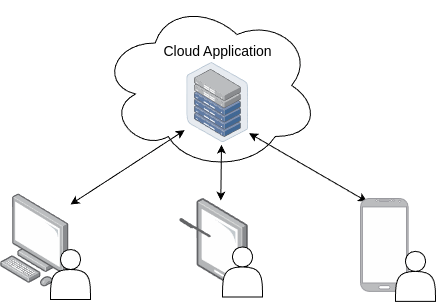
\includegraphics[scale=0.5]{images/basic-cloud-services.drawio.png}
	\caption{Users can access cloud applications from any device with an internet connection.}
	\label{fig:cloud-applications}
  \vspace{-1em} % Negative  oalue to remove space
\end{figure}

% A key selling point of these, is that companies don't have to do any technical work setting the software up, they can pay for a subscription and start using the tool right away, either through a browser or by installing an executable on their computer.
% A very important technical aspect for such tools, that enables the ease of use, is the ability to support multiple companies using them at once.

% Most of these benefits only apply if all users interact with the same cloud application.
% This means that the users interact with what appears to them to be a single application
% This is called multi-tenancy, and it is implemented by most popular cloud applications, e.g. by Teams, Slack, Asana, and many more.
% A tenant can be seen as an entity that uses the application, which can be either a single user or an organization made up of many users.

One very common feature that makes these benefits possible is called \textit{multi tenancy}.
\textit{multi tenancy} is a software architecture in which one single instance of an application
can be used by multiple users or organizations at the same time.
Without \textit{multi tenancy}, each user or organization would need to run the application on
their own computers,
negating most of the benefits listed earlier.

% means that many different users or organizations can use the same cloud application at the same
% time, even though it looks like they each have their own private version.

% NOTE: maybe take this out
Think of an application that supports \textit{multi tenancy} like a big apartment building.
Each tenant (user or organization) has their
own private apartment (their space), where they store their belongings (their assets).
Every tenant is living in the same building (cloud application), but each tenant has their
own private space.

Many popular cloud applications use this approach. For example, when you use Microsoft Teams,
Slack, or Asana, you're sharing the application with many other companies, but you only
see and interact with your own team.

\begin{figure}[H]
	\centering
	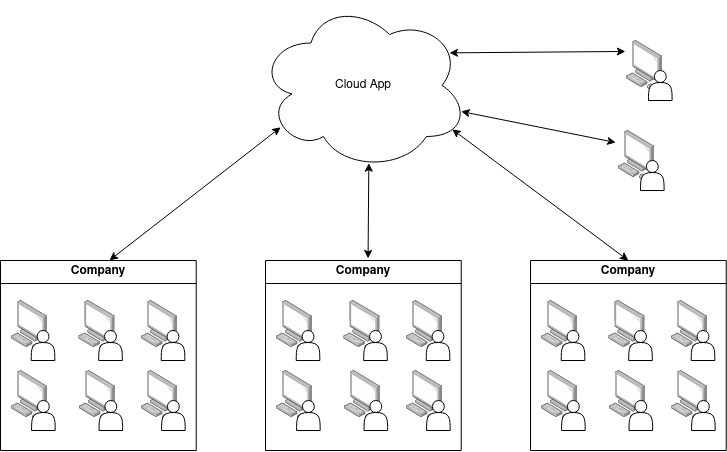
\includegraphics[scale=0.45]{images/mt-cloud-services.png}
	\caption{Multi tenancy in cloud applications: the same instance of the cloud
		application, can be used by different tenants, with different structures, without them knowing about each other.}
	\vspace{-1em} % Negative value to remove space
	\label{fig:multi-tenant=cloud-applications}
\end{figure}

PROCEED %(short for PROCess EnginE in a Distributed environment)% is a cloud application,
is a Business Process Management System,
it uses BPMN at its core to model and execute business processes.
%For readers unfamiliar with BPMN, 
%it can be thought of as a powerful flowchart that can be used to describe any conceivable process.
BPMN (Business Process Model and Notation) is a standardized graphical notation used for documenting business processes.
BPMN is typically used inside of organizations to illustrate sequences of tasks,
decision points, and interactions within various business processes, providing a standardized visual representation.

PROCEED offers two products:
\begin{itemize}
	\item Distributed Process Engine (DPE for short): the DPEs execute BPMN processes.
	\item Management System (MS for short): the MS is a cloud application that gives users
	      a graphical interface to work on their BPMN processes and deploy these to the DPEs.
\end{itemize}

\begin{figure}[H]
	\centering
	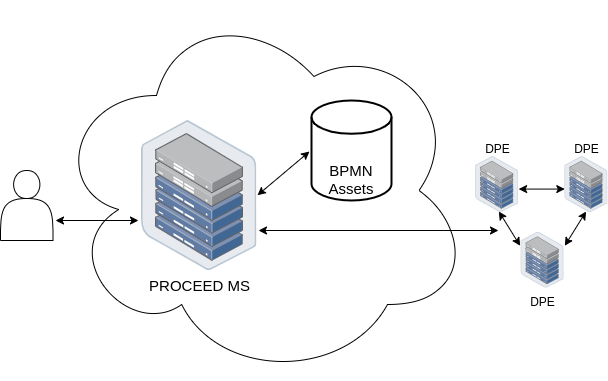
\includegraphics[scale=0.45]{images/quick-ms-overview.png}
	\caption{Overview of PROCEED: users interact with the Management System, to create and
		manage BPMN models. The Management System has the ability to deploy these models to the Distributed Process Engines.}
	\label{fig:proceed-overview}
	\vspace{-1em} % Negative value to remove space
\end{figure}

%Throughout this thesis we'll refer to any information that a user can access as an asset.
%Also all actions that a user can perform in the PROCEED Management System, are viewed as an action performed on an asset.

%The PROCEED Management system encompasses various asset types, which can be categorized as follows:
%\begin{enumerate}
%    \item BPMN models: Processes, Projects, and Templates are assets that can be created in PROCEED, that fall into the category of BPMN models.
%    Although each one of them stores slightly different information and carries a distinct semantic meanings, they all have BPMN at their core.
%    \item Execution related assets: Tasklist, Executions and Machines are all assets related to the execution of a BPMN model.
%end{enumerate}

% TODO !!

Currently the MS lacks full multi-tenancy support, it only supports individual users and
doesn't fully support organizations.
For organizations to be supported, members of the organization need to be able to have a
shared workspace, where they can work on the same assets.
% This could technically achieved if members of the organization shared all assets with
% each other.
However, PROCEED only supports universal sharing, meaning that all users would be able to
see the shared assets.
Furthermore, even if it was possible to share assets only to a group of users, it would be
very cumbersome and error-prone.
% This means that organizations, where multiple people work together are not supported by the
% MS.
% For this reason, it presents many difficulties for organizations, as there is no convenient way for multiple members of the organization to work together on assets in the MS.
% For this reason, the MS is not suitable for organizations, as there is no convenient way
% for multiple members of an organization to work together.
% Furthermore, any admin user in the MS has the right to view and modify every asset, which presents privacy risks for organizations.
% The only somewhat viable option for organizations to use PROCEED, is to run the server
% code of the MS on their own computers, which renders most benefits of cloud applications void.
%This is because all assets are stored in a central database without a good way to isolate them from other tenants.
%The only information that BPMN related assets are stored with, that helps towards isolating them from other tenants is the owner and a set of labels.

For this reason, this thesis implements multi-tenant functionality into the PROCEED MS by introducing the concept of Environments.
The MS should be able to hold multiple isolated environments, where tenants can work on their assets.
% Each tenant should be able to work in their own isolated environment, which lives in a central instance of the Management System. 
Each user, who signs in, should automatically have their own Environment, this allows users to work on
personal projects.
Organizations should be able to create environments where multiple members can work together.
Additionally, environments should include a folder structure to improve the organization of
assets.
% Currently the MS only provides labels for organizing assets.
% Assets can be labeled with one or more labels, which can be used to filter assets. 
% Users cannot add, delete nor modify these labels.
% Folders will provide more flexibility than labels.

\begin{figure}[H]
	\centering
	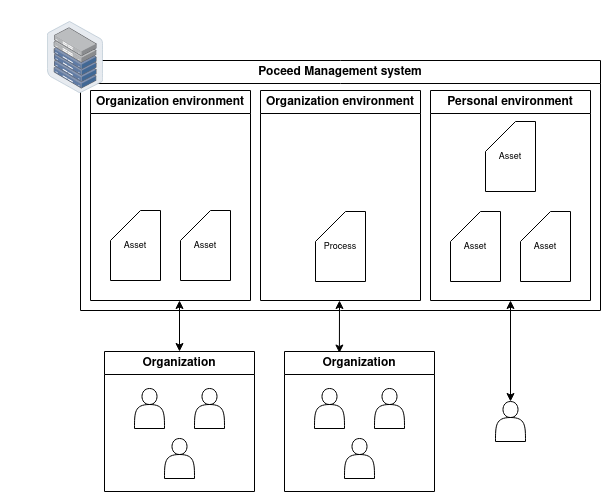
\includegraphics[scale=0.45]{images/proceed-workspaces-v2.drawio.png}
	\caption{Goal of this thesis: tenants can work in their own isolated environments in
		the PROCEED Management System.}
	\label{fig:proceed-envitonments-overview}
\end{figure}

% These labels symbolize, what department the process belongs to. 

%Access to assets in the MS is restricted through roles,
%so that one of three scenarios can happen to a user:
%
%\begin{itemize}
%    \item The user doesn't permissions to see assets.
%    \item The user has permission to view assets, but isn't an admin. In case, the user would only be able to see his own assets.
%    \item The user is an admin and can see all assets.
%\end{itemize}
%
%This low level of granularity makes the PROCEED Management System unsuitable hosting multiple tenants, since all their assets would be stored in the same fashion, and the only way for users to see assets that weren't created by them, would be to grant them the admin role.
%Granting users the admin role, would in turn mean that they would be able to see all BPMN Assets, which poses privacy concerns for tenants, since other tenants could potentially access their assets.

%When it comes to Execution related assets, Machines and Executions also have similar problems to BPMN assets, since these need to be private for each company.

%This makes it so, that if more than one tenant wants to use PROCEED they're left with few options:
%
%\begin{itemize}
%\end{itemize}
%Each company would have to spin up their own self hosted version of PROCEED.
%
%Both of these options have considerable downsides. 
%No separation between companies is a hindrance to privacy and each company having to spin up an instance of PROCEED is a big barrier to entry.
%This makes it very hard to scale PROCEED to be able to be comfortably used by multiple companies.
%
% \begin{figure}[H]
%    \centering
%    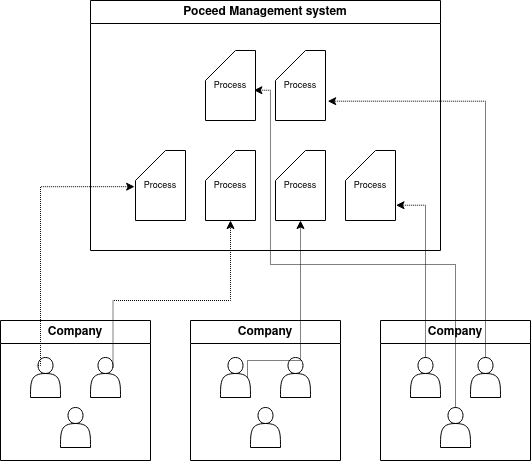
\includegraphics[scale=0.5]{./images/proceed-no-workspaces.drawio.png}
%    \caption{PROCEED Management System with no multi-tenant support.}
%    \label{fig:PROCEED-no-Environments}
% \end{figure}


% Research questions
\section{Research Questions}
\label{cha:researchquestions}

For environments to be successfully integrated into the PROCEED Management System,
a few important questions need to be addressed.
These questions will help ensure that environments work smoothly with the existing database structure,
role system, and user management. By answering them, we can ensure the implementation is effective and doesn’t
disrupt the current system.


\begin{enumerate}
	% Data Modeling and Architecture

	\item Environment representation: How can we model environments and their hierarchical
	      folder structure within the MS's storage solution to ensure the following:
	      \begin{itemize}
		      \item Data integrity: find a schema that facilitates data consistency after updates.
		      \item Asset-Environment association: find a schema that associates assets with their
		            respective environments while maintaining a clear and consistent data model.
		      \item Efficiency: find a schema that allows to efficiently query the database.
	      \end{itemize}

	\item How do users have to be managed to best allow them to be members of multiple environments?

	\item How can organizations model their hierarchical structures within environments
	      to allow members of the organization to have different levels of access to assets?
	      % \item How can we extend the existing PROCEED role system to incorporate
	      %   environment-specific permissions?

	      % Roles and Permissions
	\item How can users work on personal Projects outside an organization.


	      % \item What mechanisms are needed to ensure that role-based access control is consistently enforced?

	\item How can the Management System allow users to manage assets on different
	      environments?

	      % Usability and Developer Experience

	      % \item What user interface elements and interaction patterns are most effective for navigating and managing folders and environments?

	      % \item How can we minimize the impact on existing code while ensuring seamless integration?

	      % Additional Considerations

	      % Performance and Scalability: How will the addition of environments impact the performance and scalability of the PROCEED Management System? What optimizations can be made to ensure that the system remains responsive and efficient even with a large number of users and environments?
	      % Migration Strategies: How can we seamlessly migrate existing PROCEED data and users into the new environment-based structure? What strategies can we employ to minimize disruption during the transition?
	      % Security: What additional security measures are needed to protect data within environments? How can we prevent unauthorized access to environments and their assets?
\end{enumerate}

% Task List

\section{Task List}
\label{cha:tasklist}

The following task list outlines the concrete steps necessary to address the research
questions and ensure a successful implementation of environments.
Each task is designed to tackle specific aspects of the MS's
architecture, user management, and role assignments.

% private environment
% Functional / non functional
% can / must / should 
% TODO: 
% \item What software abstractions (e.g., classes, interfaces, functions) can we create to simplify the process of identifying and managing a user's environment in the backend code? 

\begin{enumerate}
	\item The MS has to support environments, isolated spaces where users can work on their
	      assets. \label{cha:tasklist:item-environments}
	      \begin{enumerate}
		      \item Every asset in the MS \ref{cha:relatedwork:proceed-assets} must be stored in only one environment.

		      \item Assets stored in one environment can only be accessed by members of that
		            environment.

		      \item Environments must have a hierarchical folder system to store assets.
		            \begin{enumerate}
			            \item Find a suitable abstraction to represent folders in a database
			                  that facilitates consistency after updates and is fast to query.

			            \item Ensure privacy between environments.

			                  % escribir aca ya que tiene que haber herencia
			                  % reescribir should be modified no es tan fuerte/
			                  % likely redundant

			                  % depending on the folder the asset is in.
		            \end{enumerate}

		            % NOTE: replace concurrently with eaesier word
		      \item The MS must be able to hold multiple environments and let users access them concurrently.

	      \end{enumerate}
	      % ---------------------------------------------------------------------------------------
	      % ---------------------------------------------------------------------------------------

	      %write about how there are personal and organization environments
	\item Implement personal and organization environments. While both are environments
	      and share common functionality as described in
	      \ref{cha:tasklist:item-environments}, they must behave differently in some
	      situations.
	      \begin{enumerate}
		      \item Personal environments can only have one member.

		      \item Personal environments can only store Processes and Folders.

		      \item Organization environments support all assets described in \ref{cha:relatedwork:proceed-assets}.

		      \item Organization environments can have a name and description.

		      \item Organization environments must support multiple members, i.e. multiple users can
		            work on the assets stored inside of it.

		      \item Organization environments must have a role system, where roles can be assigned to
		            users, to manage their access to assets.

		      \item Users of organization environments that have the right permissions must be able to invite users
		            to the organization environment.
	      \end{enumerate}


	\item The MS's user management has to be adapted to fit environments: before the
	      implementation of this thesis, users where strictly tied to one instance of the MS,
	      meaning each time a new instance of the MS was created, a new user storage had to be
	      configured.
	      \begin{enumerate}
		      \item Users have to be global, meaning that they don't belong to any environment.

		      \item Implement Guest users.
		            \begin{enumerate}
			            \item Allow users to try the MS without signing in with their personal
			                  information.
			            \item Guest users can sign in with their personal information and become a normal
			                  user.
			            \item Guest users can transfer their assets to a normal user.

			            \item Guest users can not create or be part of organization environments.
		            \end{enumerate}

		            % TODO: does this belong here?
		      \item Every user has to have a personal environment.

		            % TODO: does this belong here?
		      \item Personal environments must be tightly coupled with users, i.e. when a user is
		            deleted so is his personal environment.
	      \end{enumerate}


	\item The MS's preexisting role system must be adapted to fit organization environments
	      and their folder structure:
	      The MS already has a role system in place to manage users' access to resources,
	      this has to be adapted to work with organization environments.
	      \begin{enumerate}
		      \item Roles must belong to only one organization environment.
		      \item The role system must be replicated for each environment, i.e. it works the
		            same as before, with the difference that it is now specific to an environment.
		            E.g. if a role allowed a user to manage all processes before the implementation of
		            environments, now, with the same role, he will be able to modify all processes
		            inside the organization environment the role belongs to.
		      \item Find a suitable permission inheritance model for roles based on the folder
		            structure of an environment (e.g. a user with a role in a parent
		            folder, has the same permissions in all subfolders).
		      \item Ensure roles are always enforced in the backend.
		      \item The frontend UI must adapt to a user's roles, by only showing options that the user has permission to do.
	      \end{enumerate}
\end{enumerate}

The following are non-functional requirements that have to be met for the implementation
of environments in the MS.
The goal of these is to ensure that the implementation is user-friendly and most
importantly developer-friendly, as many developers will have to work with the codebase in
the future.
This means that where possible, simple solutions should be favored over complex ones.

\begin{enumerate}
	\item Keep changes to the MS to a minimum.

	      % \item The implementation shouldn't be repetitive, the same functional components should be used for both personal and organization environments.

	\item The user interface for navigating and managing folders and environments should
	      be intuitive and easy to use.

	\item Prioritize developer experience by creating clear abstractions and APIs.
	      \begin{enumerate}
		      \item The same data structure and functions should be used for both personal and organization
		            environments where possible. E.g. the same function that creates a folder in a
		            personal environment should be used to create a folder in an organization environment.

		      \item Choose a simple data structure for the folder system, with straightforward
		            functions for modification.

		      \item Create simple abstractions for the backend code of the MS, that allow to
		            acknowledge a user's environment with minimal effort.

		      \item Create a simple abstraction for the frontend, that facilitates adapting
		            the Interface for each.
	      \end{enumerate}

	      % \item Environments should be easy to create, manage and delete.
	      %   \begin{enumerate}
	      %     \item The frontend should provide intuitive interfaces for creating and deleting organization environments.
	      %       // not functional
	      %     \item Provide well documented APIs to create, manage and delete environments both for the frontend and the backend.
	      %       needs more description. ldap
	      %     \item Environments should provide the option to import an existing user database.
	      %   \end{enumerate}
\end{enumerate}



%---------------- 
% old

% \begin{enumerate}
% \item The same data structure should be used to represent personal and organization environments.
% \begin{enumerate}
% \item Personal and organization environments should have a near identical structure.
% kann man falsch verstehen umschreiben
% \item Most of the backend and frontend code should work the same, regardless of if it is dealing with a personal or an organization environment.
% \end{enumerate}

% not functional - keine stichpunkte  - : 2 points in one paragraph

% \end{enumerate}

% The introduction of "environments" within this system is a pivotal enhancement. These environments serve as distinct, isolated spaces, ensuring that the contents and operations within each environment remain entirely separate from those in all other environments. This separation offers users the capability to manage various aspects of PROCEED's functionality while maintaining data and process integrity within their designated environment. This thesis explores the design, implementation, and implications of the multi-tenant feature within the Management System of Proceed, contributing to a more versatile and secure user experience.


% \begin{enumerate}
%     \item Interface for creatring and deleting company workspaces.
%     
%     \item Adapt roles to workspaces.
%     \begin{itemize}
%         \item Each role has to belong to one workspace
%         \item Roles have to cascade down the folder structure of workspaces
%         \item Roles have to roughly keep the same functionality as before.
%     \end{itemize}
%     
%     \item Adapt asset storage for workspaces.
%     \begin{itemize}
%         \item Find a suitable solution to store assets.
%         \item Ensure privacy between workspaces.
%     \end{itemize}
%     
%     \item Adapt the Management System's API to take into account workspaces.
%     \begin{itemize}
%         \item Make sure that a the requester specifies the workspace he is referring to.
%         \item Make sure that the requester belongs to the workspace where the asset he is trying to access is located.
%         \item Implement an endpoint for users to get the workspaces they belong to.
%         \item Implement an endpoint for users to manage the workspaces they belong to.
%     \end{itemize}
%     
%     \item The Management System frontend will only have one active workspace at a time.
%     \begin{itemize}
%         \item All actions that manipulate assets, roles or create users, will be performed on the active workspace.
%         \item Only the assets of the active workspace will be shown.
%         \item There will be a clear indication of what workspace is active
%         \item There will be an easy way to switch between workspaces.
%     \end{itemize}
%     
%     \item Interfaces for managing different aspects of company workspace's members.
%     \begin{itemize}
%         \item Option for creating and deleting users.
%         \begin{itemize}
%             \item Basic creation with manual input.
%             \item Import existing user Databases.
%         \end{itemize}
%         \item Option for inviting users to the workspace.
%         \item Option to manage users' roles.
%     \end{itemize}
%     
%     \item Users should be able to share assets.
%     \begin{itemize}
%         \item Allow users to share assets with other users.
%         \begin{itemize}
%             \item A person who shares something will be referred to as a sharer and the reciepient as a sharee
%         \end{itemize}
%         \item Users will only be able to share assets if their roles allow it.
%         \item Each shared object has associated perimissions with it, which restrict the sharee's ability to access and manipulate it.
%         \item Sharees will be able to view and select all workspaces where they have at least one shared asset.
%         \begin{itemize}
%             \item Sharees sill see the folder structure of the workspace, but they won't see any of the assets in them, besides the ones shared with him
%         \end{itemize}
%         \item The frontend will implement a Interface to share assets.
%         \item The frontend will implement a Interface to manage shares.
%         \item The frontend will indicate to the sharer, in the asset overview that an asset is shared.
%         \item Users that are allowed to view an asset will also be able to see the users that it has been shared to.
%     \end{itemize}
% \end{enumerate}

\chapter{Related Work}
\label{cha:relatedwork}

\section{OAuth 2.0 and OpenID Connect}
\label{cha:relatedwork:oauth}
%TODO: fix citing

Oauth is an open standard for access delegation, 
commonly used as a way for users to grant client applications access to their information on other applications.
Oauth was born as a necessary security measure, to avoid sharing plaintext credentials between applications.
Plaintext credential sharing, as outlined in \cite{rfcOauth2} has many security risks:

\begin{enumerate}
  \item Applications are forced to implement password authentication, to support the sharing of plaintext credentials.
  \item Third party applications gain overly broad access to the user's account.
  \item Users cannot revoke access to specific third party applications.
  \item If any of the third party applications are compromised, the user's account is at risk.
\end{enumerate}

Oauth adresses these issues by decoupling the client application from the role of the resource owner,
meaning that the client application will not get a full set of permissions to the user's account.
Insetead of handing his crendentials to the third party application,
the resource owner signs in, in the application's website which then issues an access token to the client application.
This method avoids the user having to share his credentials with third party applications.

\subsection{OAuth 2.0 Roles}

Oauth 2.0 defines four roles for participants in the protocol flow:

%TODO: rewrite this, it is looking too much like the original spec
\begin{enumerate}
  \item Resource owner: The entity that can grant access to a protected resource, typically this would be an end user of a web application.
  \item Resource server: The server hosting the protected resources.
  \item Client: The application requesting access to the protected resources. 
    OAuth 2.0 distinguishes between two types of clients: confidential and public clients.
    Confidential clients are capable of keeping their credentials confidential, while public clients, like browser-based applications, cannot.
  \item Authorization server: The server that issues access tokens to the client after the resource owner has been succesfully authenticated.
\end{enumerate}

The resource server and the authorization server can be the same entity, but they are not required to be.

\subsection{Authorization Grants}

%TODO: public and private client
%TODO: authorization tokens

Authorization Grants are credentials that are issued to clients, which can be exchanged for an access token.
This access token can be used to access the protected resources on the resource server.
Oauth 2.0 defines four authorization grants with different flows.

%TODO: footnote for http redirects or smthing

\subsubsection{Implicit}
\label{cha:relatedwork:oauth:implicit}

% The implicit grant is a simplified version of the Authorization Code grant.
The implicit grant is very helpful for public clients, as it doesn't require confidential client credentials.
This is very helpful for browser-based clients, as they can't store confidential credentials securely.
In the implicit grant users are redirected to the authorization server, where they authenticate thmeselves and authorize the client.
Afterwhich the authorization server issues an access token directly to the client,
this is done so with a HTTP redirect, where the access token is embedded in the redirect URL,
this way the client can extract the access token from the URL.
% The access token gets embedded in the redirect URL, after the resource owner was authenticated, which is then sent to the client.

In this flow the resource owner only authenticates with the authorization server, 
thus never having to share his credentials with the client.

Implicit grants have many security risks, as the access token is exposed in the URL and can be intercepted by a malicious attacker.
This is why PKCE (Proof Key for Code Exchange) was later introduced as an addition to the implicit grant \cite{rfcPkce}.

\subsubsection{Resource Owner Password Credentials}
\label{cha:relatedwork:oauth:passwordcredentials}

This grant type requires the resource owner to share his password credentials with the client.
The resource owner's password credentials represent an authorization grant,
which the client can exchange them for an access token.
Even though this grant type requires the resource owner to share his credentials with the client,
these are only used for one request and don't have to be stored.


\subsubsection{Client Credentials}
\label{cha:relatedwork:oauth:cleintcredentials}

The client credentials grant is used when the client is the resource owner.
Clients are typycally issued crendentials, which they can use to authenticate themselves.
Clients send these credentials to the authorization server and are issued an access token.

\subsubsection{Authorization Code}
\label{cha:relatedwork:oauth:authcode}

The Authorization Code grant is the most common grant type used in OAuth 2.0,
it is similar to the implicit grant \ref{cha:relatedwork:oauth:implicit}, as it also uses HTTP redirects and it doesn't require the resource owner to share his credentials with the client.
In the authorization code grant, the client redirects the resource owner to the authorization server.
There the resource owner authenticates himself and authorizes the client.
afterwhich the authorization server redirects the resource owner back to the client with an authorization code.
The client then authenticates itself with his confidential credentials on the authorization server and exchanges the authorization code for an access token.
As the client needs confidential credentials, this flow is only suitable for confidential clients.
The exact steps are shown in figure \ref{fig:oauth:authcodeflow}.

\begin{figure}[H]
    \centering"
    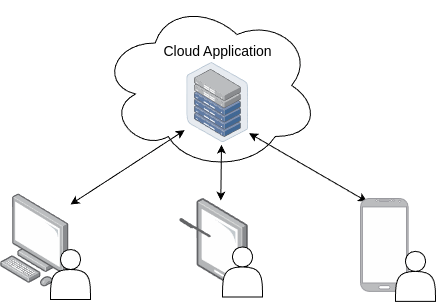
\includegraphics[scale=0.4]{images/basic-cloud-services.drawio.png}
    \caption{Cloud Application.}
    \label{fig:oauth:authcodeflow}
\end{figure}

\subsection{OpenID Connect}
\label{cha:relatedwork:openid}

\section{PROCEED's role system}
\label{cha:relatedwork:proceedroles}

The PROCEED MS uses a Role-Based Access Control (RBAC) system to mange user authorization,
i.e. to determine what actions a user can perform.
Roles can be seen as bundles of permissions, which are granted to users.
A user can have multiple roles.
Typically roles are assigned to users based on their job function.
%% Advantages 
%% - One role serves multiple people
%% - roles don't change ofte
%% - roles are easier to manage than individual permissions
RBAC can be advantageous since they can be assigned to multiple users and 
don't change often, making them easier to manage than individual permissions.

\subsection{MS's Role System Terminology}
\label{cha:relatedwork:proceedroles:terminology}

The following terms are important to understand the role system in the PROCEED MS:

\begin{itemize}
  \item Resource: A resource is any protected entity in the management system, that can be
    accessed by users.
  \item Action: An action is a specific operation that can be performed on a resource.
  \item Permission: A permission is a tuple of resource type and action, which specifies that a
    user can perform the action on the resource instances. Optionally a permission can have
    conditions that have to be met the by resource instances, for the user to be able to perform the action.
  \item Role: A role is a set of permissions. Roles can be assigned to users, which then
    inherit the role's permissions. Roles can have expiration dates, after which all
    permissions are revoked.
\end{itemize}

\subsection{MS's resources and actions}
\label{cha:relatedwork:proceedroles:ms-resources-actions}

The following are the resource types that are used in the PROCEED MS:
  \lstinline{Process}, 
  \lstinline{Project},
  \lstinline{Template},
  \lstinline{Task},
  \lstinline{Machine},
  \lstinline{Execution},
  \lstinline{Role},
  \lstinline{User},
  \lstinline{Setting},
  \lstinline{EnvConfig},
  \lstinline{RoleMapping},
  \lstinline{Share},
  \lstinline{Folder}.

These are the actions that can be performed on these resources:
  \lstinline{none},
  \lstinline{view},
  \lstinline{update},
  \lstinline{create},
  \lstinline{delete}.

\subsection{MS's roles in CASL}
\label{cha:relatedwork:proceedroles:casl}

The PROCEED MS uses \footnote{https://casl.js.org/v6/en/}{CASL} to implement Rules. CASL
is an isomorphic authorization JavaScript library.
To enforce authorization CASL has abilities, which are assigned to users.
Abilities expose functions to check weather a user can perform an action on a resource.
Abilities are defined by four parameters: user action, subject, fields, conditions.
User actions and subjects are analogous to actions and resources \ref{cha:relatedwork:proceedroles:terminology}.

CASL differentiates between subject type and subject instance. 
A subject instance is a specific instance of a subject type, e.g. a specific process
users are working on, is an instance of the resource type "Process". 

Fields are used to specify which fields of a resource instance an action can be performed
on, e.g. a user can update a process's name, but not its id, or creation date.

Conditions are used to specify additional conditions that have to be met by a resource
instance, for a user to be able to perform an action on it. E.g. a user can only update a
process if he created it.

\begin{lstlisting}[
  language=Javascript,
  style=codestyle,
  caption={CASL example},
]
import { defineAbility } from '@casl/ability';

class User {
  constructor(id) {
    this.id = id;
  }
}

class Process {
  constructor(user, name) {
    this.authorId = user.id;
    this.createdOn = new Date();
    this.name = name
  }
}

function abilityForUser(user){
  return defineAbility((can, cannot) => {
    can('delete', 'User', {id: user.id});

    can('update', 'Process', ['name'], {authorId: user.id});
  });
}

const user1 = new User(1);
const user1Ability = abilityForUser(user1);
const user1Process = new Process(user1, 'some process');

const user2 = new User(2);
const user2Ability = abilityForUser(user2);

user1Ability.can('update', 'Process'); // true
user1Ability.can('update', user1Process, 'name'); // true
user1Ability.can('update', user1Process, 'createdOn'); // false

user1Ability.can('delete', user1); // true
user1Ability.can('delete', user2); // false

user2Ability.can('update', 'Process'); // true
user2Ability.can('update', user1Process); //false
\end{lstlisting}

If there exist any possible resource instance, where the user has permission to perform an action,
then the user has permission to perform the action on the resource type.
E.g if a user has permission to view some process in the MS, then he has permission to view .

\chapter{Concept and Design}
\label{cha:conceptanddesign}

This chapter outlines the key components of the implementation of environments in the MS.
The core components are users, environments, roles, and assets.
In essence the concept can be summarized as follows: users can be part of multiple
environments, which hold Assets.
Users that are part of an environment can work on the assets that are stored in it.
Each environment has a set of Roles that determine what their users can do with its
assets.
All other components that will be introduced will help to manage and enforce these relationships.

\section{Modifications to Assets and Resources}

This thesis will modify all assets and management assets \ref{cha:relatedwork:proceed-assets}
that are supported by the MS,
these will be modified to be contained inside environments.
Additionally, environments will be added to the MS' assets and resources.
As will be explained in \ref{cha:conceptanddesign:users}, Users won't belong to a single
environment, they can instead be members of multiple environments, for this reason,
users will be removed from the MS' assets and resources.
Furthermore, folders and  memberships will be added to the MS' assets and
resources.

\section{Data Storage Approaches for Isolated Environment Data}

As outlined in \cite[3.3]{multi-tenant-dream-or-nightmare},
data leaks between tenants are very dangerous.
For this reason isolation between tenants is crucial.
The first step to ensure isolation is to choose a good data storage model.
There are mainly three models to choose from as described in
\cite[4.1]{Pushpan2024MultiTenantArchitecture}:

\begin{itemize}
  \item \textbf{Separate databases}: Each tenant has a dedicated database instance,
    offering complete physical isolation.
    This model offers a high isolation level,
    however it is resource-intensive and it involves a high operational overhead.

  \item \textbf{Shared database, separate schemas}: All tenants share the same database, but each has a distinct schema. 
      This approach balances isolation and resource efficiency, with less complexity than fully separate databases.

  \item \textbf{Shared database, shared schema}: All tenants use the same database and schema, with tenant data identified by a tenant ID. This model maximizes resource efficiency but requires robust access control and query isolation mechanisms to ensure tenant boundaries are respected.
\end{itemize}

% Since the MS currently uses JSON files as its storage system,
% separate databases and separate schemas would come down to storing each environment's data
% in different files.
% I kinda think multiple files would be good, like for cache layers, where a table leads
% to another, too bad :/ 
% TODO: kai wants a better explanation of why I chose the third model
Since the first two models are resource-intensive and introduce operational
overhead, we chose the third model: \textbf{Shared database, shared schema}.
The trade-off is a lower level of data isolation compared to the other two approaches.
To mitigate this, every asset in the system explicitly stores an \lstinline{environmentId},
which is always validated during data access and modification operations.
This strict enforcement ensures tenant boundaries are always respected.


\section{New User Management System}
\label{cha:conceptanddesign:users}
%NOTE: maybe change the sctructure of this paragraph a bit

Previously all users in the MS were members of a single organization.
In order for users to be part of multiple organizations, they can't be tied to a single
organization.
As a part of the implementation of environments, users are now independent of
organizations,
they represent individual people utilizing PROCEED and are stored as entries in
the MS' storage solution.
% A single person can have one or more users, but each user is intended for individual use.

To facilitate the exploration of the MS, without creating a user, we introduced the option
to use the MS as a guest.
Thus, we differentiate between authenticated users and guest users.
Guest users can only use a subset of the MS' features.
Guest users can transition to being authenticated users whilst retaining their
assets, to do this they will need to sign in with their personal data.
% Creating a Guest user doesn't require any data from the person creating it.

All users have a personal environment \ref{cha:conceptanddesign:environments:personal}
in which they can create and manage assets freely.
Authenticated users can also be part of and create organization environments
\ref{cha:conceptanddesign:environments:organization},
where they can collaborate with other users.

\subsection{Authenticated Users and Accounts}

% NOTE: is Oauth2 account the correct term here?
To allow the same user to be able to sign in with different Oauth 2.0 providers, e.g. with
Google or Facebook,
we store a separate record, called \textit{account}, for each of the user's sign-in methods.
This means, that the relationship between users and accounts is one-to-many,
a user can have multiple accounts, but an account can only be linked to one user.
When a user signs in with a Oauth 2.0 provider, the provider returns a user ID, 
then the MS searches for an account with the same user ID.
From that account the MS can find the user.
% This way, when a user is signing in with credentials from a Oauth 2.0 provider,
% the MS can look up the corresponding account to the account returned by the provider, and then find the user
% that the account is linked to.

\begin{figure}[H]
	\centering
	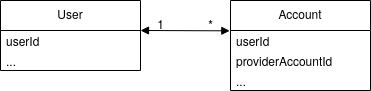
\includegraphics[scale=0.6]{images/users-accounts-relation.drawio.png}
	\caption{Relation between users and accounts.}
	\vspace{-1em} % Negative value to remove space
\end{figure}
% caption: Relationship between users and accounts.

\subsection{Merging a Guest User with an Authenticated User}
\label{cha:conceptanddesign:users:mergeguestuser}

As previously stated, a guest user can transition to being an authenticated user by
signing in with his personal data.
Afterward the user will be marked as authenticated and will be able to use the MS freely.
However, it could be the case that his personal data already corresponds to an existing user.
In this case, the user will be asked if he wants to merge his assets with the existing
authenticated user.
If he chooses to do so, all the assets in the guest user's personal environment will be
transferred to the authenticated user's personal environment.
Otherwise, all the assets created by the guest user will be deleted.

%TODOFIG: make flow clear

\subsection{Guest User Storage}
\label{cha:conceptanddesign:users:guestuserstorage}

For storing guest user data, one could take one of two approaches:
storing the data in the user's browser or storing it in the MS' database, alongside the
data of authenticated users.
Storing the data locally has two benefits:
The MS doesn't have to store data of users who might never return and
the MS would become less susceptible to an attack where the attacker tries to use up as
much space as possible in the MS' storage solution.
However, this approach has one key downside, the MS would have to implement two storage
solutions and the frontend would need to switch accordingly between them.
The added complexity would make it harder for developers to get an overview of the MS'
codebase and it would mean that any future changes will have to be implemented twice.
% and it also makes it harder to use coding assistance features of IDEs like Goto
% definition \footnote{\url{https://microsoft.github.io/language-server-protocol/specifications/lsp/3.17/specification/\#textDocument_definition}}.
For this reason, we determined that storing guest user's data locally isn't worth the benefits.
We decided to store guest users data in the MS the same way we do it for
authenticated users,
with the difference that a flag is set
in the user entry to indicate that they are a guest.
This way, all the endpoints that authenticated users can call to interact with the MS
can also be called by guest users.
An important caveat is that, to enforce some of the feature restrictions, relevant
endpoints have to check whether the user is a guest.
Furthermore, the MS needs to clean up inactive guest users, to prevent the MS' storage
solution from filling up with unused data.

\subsection{Development Users}

During development, it is often inconvenient or impractical for developers to configure all the necessary environment variables required for full authentication functionality.
For instance, integrating OAuth 2.0 authentication (see Section \ref{cha:relatedwork:oauth}) or enabling email-based sign-in requires valid credentials, secrets, and sometimes external services that may not be accessible in a local development environment.

To streamline testing and development without depending on such services,
the Management System (MS) implements two predefined development users: \textit{johndoe} and \textit{admin}.
These users are only available when the MS is running in a development environment.

%TODO: say what guests can do?

% NOTE: I think this goes in implementation
% \subsection{Accounts}
%
% Accounts represent a use's sign in method. 

\section{Hierarchical Folder Structure}
\label{cha:conceptanddesign:folders}

Folders will be added to the MS' assets,
they are intended to allow organizations to mirror their hierarchical structure and
to facilitate the organization of assets in general.
Starting from a root folder, users are able to store assets within folders and nest
folders inside other folders, creating a flexible and intuitive structure.
In this thesis, folders were only implemented to support processes, but they could be extended to
support more of the assets that were described in \ref{cha:relatedwork:proceed-assets}.

\subsection{Folder Structure Storage Model}

% TODO: say that because of the way the ms is built, the processes needs to be in a
% sepparate table

The folder structure is essentially just a rooted tree.
The MS doesn't use a database management system, thus it doesn't use a relational
language like SQL, still, the data is stored in a way that mimics a relational model.
For this reason the rooted folder tree needs to be mapped to a relational model.
% Methods mentioned in book
%
% Materialized path
% Nested sets -> store leftmost and rightmost of set
% Interval halving
% Matrix encoding
% Nested intervals
As outlined by Joe Celko in \cite[28]{celkoSQLTrees}, there are mainly three ways to model
trees in relational model:
Adjacency List, Nested Set, and  Path Enumeration, more commonly known as Materialized Path.
Each of these models stores a node as a single entry, but they differ in how they encode
their position in the tree:

% Categories
% 1. finding direct descendandts / children
% 2. finding nth descendandts
% 3. finding ancestors / parent
% 4. finding nth ancestors
% 5. Adding
% 6. removing
% 7. Reorganization

\begin{itemize}[nolistsep]
	\item \textbf{Adjacency List model}: Each node stores an identifier and a reference to its parent.
	      \begin{itemize}
		      \item Advantages
		            \begin{itemize}
			            \item Finding a node's children is trivial.
			            \item Finding a nodes' parent is trivial.
			            \item Adding a node to the tree is trivial and doesn't require updating other
			                  nodes.
			            \item Moving nodes and their subtrees is trivial, since it only requires updating
			                  the parent reference. However, a check has to be made to ensure that the node's
			                  new parent isn't one of its descendants, thus creating a cycle.
		            \end{itemize}
		      \item Disadvantages
		            \begin{itemize}
			            \item Finding a node's descendants requires a recursive query, however,
			                  this is bounded by the depth of the tree and the amount of nodes.
			            \item Finding a node's ancestors, i.e. all the nodes in the path from the root to
			                  the node, requires a recursive query, however, this is bounded by the height of
			                  the tree and should be fairly efficient.
			            \item Removing a node requires a recursive query to also delete its descendants,
			                  however, this is bounded by the depth of
			                  the tree and the amount of nodes.
		            \end{itemize}
	      \end{itemize}
	      %-----------------------------------------------------------------------------------------------------------
	      %-----------------------------------------------------------------------------------------------------------
	\item \textbf{Nested Set model}: Each node has a left and right value, describing an
	      interval starting from the left value and ending at the right value.
	      Children nodes' intervals are contained within the parent's interval. Furthermore, the
	      intervals of siblings are disjoint.
	      \begin{itemize}
		      \item Advantages
		            \begin{itemize}
			            \item Finding the descendants of a node is trivial, the query has to select all
			                  nodes, whose interval is contained within the node's interval.
			            \item Finding a node's ancestors is trivial, the query has to select the all the
			                  nodes with a left boundary smaller than the node's left boundary.
			            \item Finding a node's parent is trivial, the query has to select the node with
			                  the smallest left boundary that is smaller than the node's left boundary.
			            \item Deleting a node and its subtree is trivial, the query is analogous to finding
			                  the descendants of a node.
		            \end{itemize}
		      \item Disadvantages
		            \begin{itemize}
			            % No se si me creo esta explicacion
			            \item Finding a node's children requires a complex query, since it has to select
			                  only the node's children without also including the descendants of the
			                  children. This query can be inefficient because it has to apply additional filtering
			                  to retrieve only the direct children. This adds complexity and can slow down
			                  performance.
			            \item Adding nodes is non-trivial, since it requires knowledge of its siblings to
			                  avoid overlapping intervals. Additionally depending on the implementation, it
			                  might require updating intervals of other nodes.
			            \item Moving nodes and their subtrees is non-trivial and inefficient, since it requires updating
			                  the intervals of the moved node and all of its descendants.
			                  Depending on the implementation it may even be required to update the intervals of
			                  other nodes.
		            \end{itemize}
	      \end{itemize}
	      %-----------------------------------------------------------------------------------------------------------
	      %-----------------------------------------------------------------------------------------------------------
	\item \textbf{Materialized Path model}: Each node stores the path from the root to itself.
	      \begin{itemize}
		      \item Advantages
		            \begin{itemize}
			            \item Finding a node’s ancestors or its parent is trivial, since the path is explicitly stored,
			                  the ancestors of a node can be retrieved simply by parsing the stored path.
			            \item Finding a node’s descendants is trivial, they can be found by
			                  querying for nodes whose paths start with the current node's path.
                        However, depending on the implementation, checking each node's path can be inefficient.
			            \item Adding nodes is trivial, as the node's path can be constructed by appending
			                  the node's identifier to the parent's path.
			            \item Removing a node and its subtree is trivial, as the node's descendants can be
			                  easily queried.
		            \end{itemize}
		      \item Disadvantages
		            \begin{itemize}
			            % \item Finding a node's children is easy but, not as efficient as finding its
			            %       descendants, as you need to perform one additional check to ensure that nodes
			            %       are direct children.
			            \item Moving nodes and their subtrees is inefficient, since it requires updating
			                  the path of every node in the subtree.
			            \item Each node stores a string with its path, which can be inefficient in terms of
			                  storage space, especially for trees with a large depth.
		            \end{itemize}
	      \end{itemize}
\end{itemize}

For an example of the three models, see Figure \ref{fig:comparison-db-tree-models-pic}.
A simple comparison of these models is presented in Figure \ref{fig:comparison-db-tree-models}.

% TODO: figure out spacing
\begin{figure}[H]
	\centering
	\label{fig:comparison-db-tree-models-pic}
	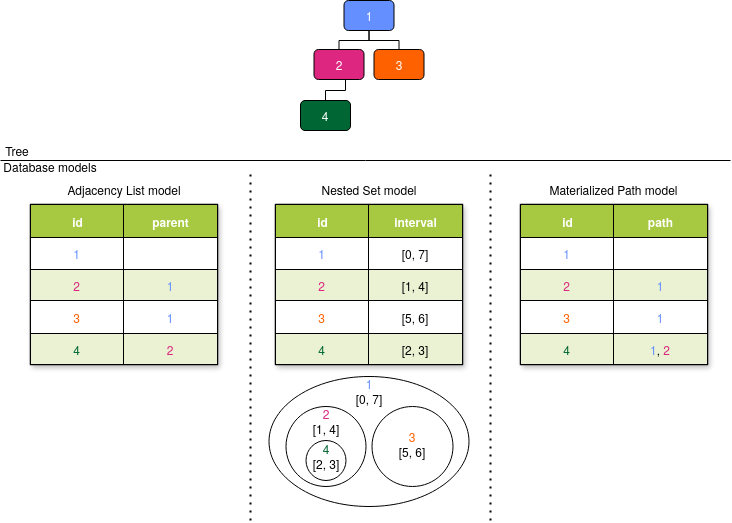
\includegraphics[scale=0.6]{./images/tree-map.drawio.png}
	\caption{Comparison of the Adjacency List, Nested Set, and Materialized Path models.}
\end{figure}

% It is worth noting, that for each of these models, we will have to sepparately delete all
% processes that are stored in the folder
\definecolor{darkgreen}{rgb}{0.0, 0.45, 0.0}
\newcommand{\goodcomplexity}[1]{\vspace{.4em}\textcolor{darkgreen}{\checkmark}\vspace{.4em}}
\newcommand{\mediumcomplexity}[1]{\vspace{.4em}\textcolor{orange}{\textcircled{}}\vspace{.4em}}
\newcommand{\badcomplexity}[1]{\vspace{.4em}\textcolor{red}{X}\vspace{.4em}}

\newcommand{\goodefficency}[1]{\textcolor{darkgreen}{\checkmark}}
\newcommand{\mediumefficency}[1]{\textcolor{orange}{\textcircled{}}}
\newcommand{\badefficency}[1]{\textcolor{red}{X}}

\begin{figure}[H]
	\centering

	\begin{tabular}{ | m{7.45em} | m{7em} | m{7em} | m{7em} | }
		\hline
		                                                               & Adjacency List                                                    & Nested Set              & Materialized Path \\
		\hline
		% ------------------------------------------------------------------------------
		find children                                                  & \goodcomplexity{Easy} \goodefficency{efficient}                   &
		\badcomplexity{Complex} \badefficency{inefficient}             & \goodcomplexity{Easy}
		\mediumefficency{somewhat inefficient}                                                                                                                                           \\
		\hline
		% ------------------------------------------------------------------------------
		find descendants                                               & \goodcomplexity{Easy} \mediumefficency{somewhat inefficient}      &
		\goodcomplexity{Easy} \goodefficency{efficient}                &
		\goodcomplexity{Easy} \goodefficency{efficient}                                                                                                                                  \\
		\hline
		% ------------------------------------------------------------------------------
		find parent                                                    & \goodcomplexity{Easy} \goodefficency{efficient}                   & \badcomplexity{Complex}
		\badefficency{inefficient}                                     & \goodcomplexity{Easy}  \goodefficency{efficient}                                                                \\
		\hline
		% ------------------------------------------------------------------------------
		find ancestors                                                 & \goodcomplexity{Easy} \goodefficency{efficient}                   &
		\goodcomplexity{Easy} \goodefficency{efficient}                & \goodcomplexity{Easy}
		\goodefficency{efficient}                                                                                                                                                        \\
		\hline
		% ------------------------------------------------------------------------------
		add nodes                                                      & \goodcomplexity{Easy} \goodefficency{efficient}                   &
		\badcomplexity{Complex} \mediumefficency{possibly inefficient} & \goodcomplexity{Easy
		and} \goodefficency{efficient}                                                                                                                                                   \\
		\hline
		% ------------------------------------------------------------------------------
		remove nodes                                                   & \goodcomplexity{Easy} \mediumefficency{somewhat inefficient}      &
		\goodcomplexity{Easy} \mediumefficency{possibly inefficient}   &
		\goodcomplexity{Moderately complex} \goodcomplexity{somewhat inefficient}                                                                                                        \\
		\hline
		% ------------------------------------------------------------------------------
		move node                                                      & \goodcomplexity{Easy} \goodcomplexity{efficient}                  & \badcomplexity{Complex}
		\badefficency{inefficient}                                     & \mediumcomplexity{Moderately complex} \badcomplexity{inefficient}                                               \\
		\hline
		% ------------------------------------------------------------------------------
	\end{tabular}

	\vspace{.5em}

	\begin{tabular}{r@{: }l r@{: }l r@{: }l}
		\goodcomplexity{\textcircled{}}\vspace{-.8em} \_ & Easy query                        & \mediumcomplexity{}\vspace{-.8em} \_ &
		Moderately complex query                         & \badcomplexity{}\vspace{-.8em} \_ & Complex query                          \\

		\_ \goodefficency{\textcircled{}}                & Efficient                         & \_ \mediumefficency{}                &
		Moderately efficient                             & \_ \badefficency{}                & Inefficient                            \\
	\end{tabular}


	\caption{Comparison between Adjacency List, Nested Set and Materialized Path models.}
	\label{fig:comparison-db-tree-models}
\end{figure}

To choose the right model, we have to consider the requirements of the MS.
Users need to be able to view, add, delete and remove folders.
It becomes immediately clear, that the Nested Set model is not suitable for the MS, as
adding, removing and moving nodes is inefficient, this model is more suited for read-heavy
workloads.
% The nested set model appears to be more useful for some analytical workloads.
That leaves us with the adjacency list and materialized path models.
%
The materialized path model has two small advantages: finding descendants and removing a
folder together with its subtree is easier.
Both queries only require simple string comparisons.
%
% The materialized path model has two small advantages, finding descendants is easier as it
% only requires a query with a simple string comparison, and the same goes for removing a
% folder and its subtree. 
%
However, the adjacency list model isn't far behind on those two points, and is
substantially more efficient when it comes to moving nodes.
Furthermore, the adjacency list model is better at finding children, which is more
valuable to the MS than finding descendants, as the Process view will only show the
children.
Additionally, the adjacency list model is more space-efficient, as it doesn't store its
path, this can be important for trees with a large depth.
For these reasons, the MS will use the adjacency list model to store the folder structure.

\subsection{Storing Assets Inside Folders}

After the folder structure is implemented, it is necessary to store assets inside
folders.
This thesis only implemented this feature for processes, however, the same principle could
be applied for other assets.
A complete redesign of the process' data structures isn't feasible, as it would require
rewriting a large part of the MS.
For this reason a simple expansion to the data structure was chosen, were analogous to
the adjacency list model, each process stores a reference to the folder it is stored in.
This approach allows a folder to be moved without requiring updates to its descendants.
Additionally, moving an asset to another folder only requires updating the asset's
reference to its folder.

% Folders are nodes in a rooted tree structure with a name and a description.
% Folders can contain other folders and assets.

% Each environment will have a folder structure to store its processes.
% The root folder is created when the environment is created.
% Each root folder and all of its children are contained by one and only one environment \ref{cha:conceptanddesign:environments}.


% Since the root folder belongs to only one environment, and all folders are stored below
% one root folder, all folders belong to only one environment.
% Processes will then store a reference to the folder they're stored in.

% TODO: ask kai if I should explain rooted trees - would be nice to cookup a formal def


\section{Environments}
\label{cha:conceptanddesign:environments}

Conceptually, environments are where everything except users are stored.
Users aren't stored in environments as they can be a part of multiple environments.
Instead, the MS stores memberships, which specify that a user is part of an environment.

There are two types of environments, personal and organization environments.
Personal environments are intended for personal use and organization environments are intended
for organizations.

\subsection{Personal Environments}
\label{cha:conceptanddesign:environments:personal}

Personal environments are assigned to each user once they sign in.
%NOTE: remove the part with owner?
The user for which the environment is created is the only member of this
environment, and is therefore called the owner.
No other users can be a part of this environment.
Personal environment only allow users to create and manage processes and folders,
while other features offered by the MS can only be used in organization environments
\ref{cha:conceptanddesign:environments:organization}.

\subsection{Organization Environments}
\label{cha:conceptanddesign:environments:organization}

Organization environments are intended to be used by organizations, thus they can have a
name, description and a logo.
In contrast to personal environments, users are allowed to use all the MS' features in
an organization environment.

% They extend the feature set of personal environments, the enabled
% resources \ref{cha:relatedwork:proceedroles:ms-resources-actions} for organization
% environments can be determined when deploying a MS instance.

Organization environments can also have multiple Users that are part of it, these are
called members.

\subsection{Environment Memberships}
\label{cha:conceptanddesign:environments:memberships}
% TODO: maybe merge this with the role stuff
% to do that however, roles would have to be added to the environment section, and I dont
% know if that's the right choice as it is a big topic

To keep track of which users are part of an environment, a new management asset will be
added: memberships.
Each membership links one user to one environment, specifying that the user is part of
that environment.

\subsection{Storing Assets inside Environments}
\label{cha:conceptanddesign:environments:storing-assets}

As previously stated, all assets within the MS \ref{cha:relatedwork:proceed-assets}, including folders,
will be modified, so that each asset instance establishes a clear association with a single environment.
Every asset will store a reference to the environment it belongs to.
This reference is immutable, with the only exception being when assets are transferred
from a guest user to an authenticated user \ref{cha:conceptanddesign:users:mergeguestuser}.

Processes and folders will be contained within folders, which implies that they belong to
the same environment as their root folder.
This means that for these assets, we are storing the environment they belong too twice.
Storing redundant information is risky as it can lead to inconsistencies if updates aren't
done correctly.
For instance if a folder's environment reference is changed, but those of its children
are not, then the folder structure would span across two environments.
However, this is not a practical issue in our implementation for two reasons.
First, an asset's environment reference is
never changed after creation, so there’s no risk of an update causing an in inconsistent
state.
Second, the only exception to this, is when the reference is modified is during the transition from a
guest user to an authenticated one, which involves transferring all the user's assets.
Outside this specific case, the remains constant, ensuring structural consistency.

% The key principle is that every asset belongs to one and only one environment, and this
% association can be easily identified.

% All of the MS' assets will only change in one way, they will somehow linked to an
% environment and only one.
% For processes, they're contained in a folder, such that they clearly belong to one
% environment. for other assets, they will store a reference to the environment they belong
% to.
% The important part is that each asset belongs to exactly one environment, and this
% environment can be identified.



\subsection{Environment Selection}
% TODO: maybe back this up with some research, although this isn't that kind of thesis

Users can be members of multiple environments and must be able to work within each of them.
There are two ways of accomplishing this: users can select one environment at a time,
or they can work on multiple environments at the same time.
%
% As environments contain many features, it isn't feasible to show all of them at the same
% time, as this would clutter the interface, some level of selection is necessary.
%
Environments contain many features and views, making it unfeasible to show them all
simultaneously for many environments.
Thus, some level of selection is necessary to avoid cluttering the interface.

%
This selection could be granular, where the user selects per view which environment he
wants to work on, however this could lead to confusion, if the user switches views and
forgets that he's working on a different environment.
For this reason, we chose to have a global environment selection, i.e. all the elements in
the UI will show the assets and views of one environment.

The environment selection can be either implicit or explicit.
In the implicit method, the selected environment is not
reflected to the user in the URL, this could be accomplished by storing the selected
environment in the user's cookies or in the browser's local storage for example.
In the explicit method, the environment is encoded in the URL,
making the current environment clearly visible.
Of course a combination of both methods is also possible, but in order to keep the
implementation simple, we will only choose one.
The implicit method has the advantage that the URLs are shorter and easier to read,
however it has the disadvantage, that some URLs can't be shared, since the implicitly
selected environment of another user might not be the same.
For this reason, the explicit method was chosen as it allows users to share links with the
cost of longer URLs and because it's more transparent to the user.

\section{Role Based Access Control within Environments}
\label{cha:conceptanddesign:roles}

% Roles are used to determine what a user can do with an asset. 
% Before the implementation of this thesis, roles in the MS
% \ref{cha:relatedwork:proceedroles} were global,
% meaning that their permissions applied to all assets in the MS.
% With the introduction of environments and the folder structure, this no longer makes sense.
% Roles will be modified to be associated with one organization environment, and they will only apply to
% the assets in that organization environment.
% In personal environments, there is only one user, and he can perform all actions on all of
% his assets.
Roles define what actions a user can perform on assets.
Prior to the changes introduced in this thesis,
roles in the MS \ref{cha:relatedwork:proceedroles} were global,
meaning their permissions applied universally to all assets across the system.
However, with the addition of environments and a folder structure, this approach is no
longer practical.
Roles will now be tied to a specific organization environment,
restricting their permissions to assets within that particular environment.
In personal environments, where there is only one user, the user will have
full control and be able to perform all actions on his assets without restrictions,
this is done internally by giving the user a role that has all permissions.

Folders allow organizations to mirror their hierarchical structure, but this wouldn't be
entirely useful if roles were applied to all assets inside the environment.
For this reason, roles can now be associated to a folder.
%
A role can define permissions for many assets, of which not all can be stored in folders.
If a role is associated with a folder, then, only the permissions that are for assets that
can be stored in folders, will be affected by this association.
% The permissions of the role that apply to assets that can be stored in folders, 
% will only apply to the assets that are in the folder's subtree.
%
The permissions of roles that are associated with a folder cascade down the
folder structure, i.e. the permissions of a role associated to a folder will 
apply to all the descendants of that folder.
In this thesis, the folder structure was only implemented for processes,
this means that only the permissions for processes and folders will 
cascade down the folder structure.
Roles that aren't associated to a folder will be applied to all assets in the environment.
% As roles are meant to mirror a users position in an organization, they're only available
% for organization environments.

\begin{figure}[H]
	\centering
	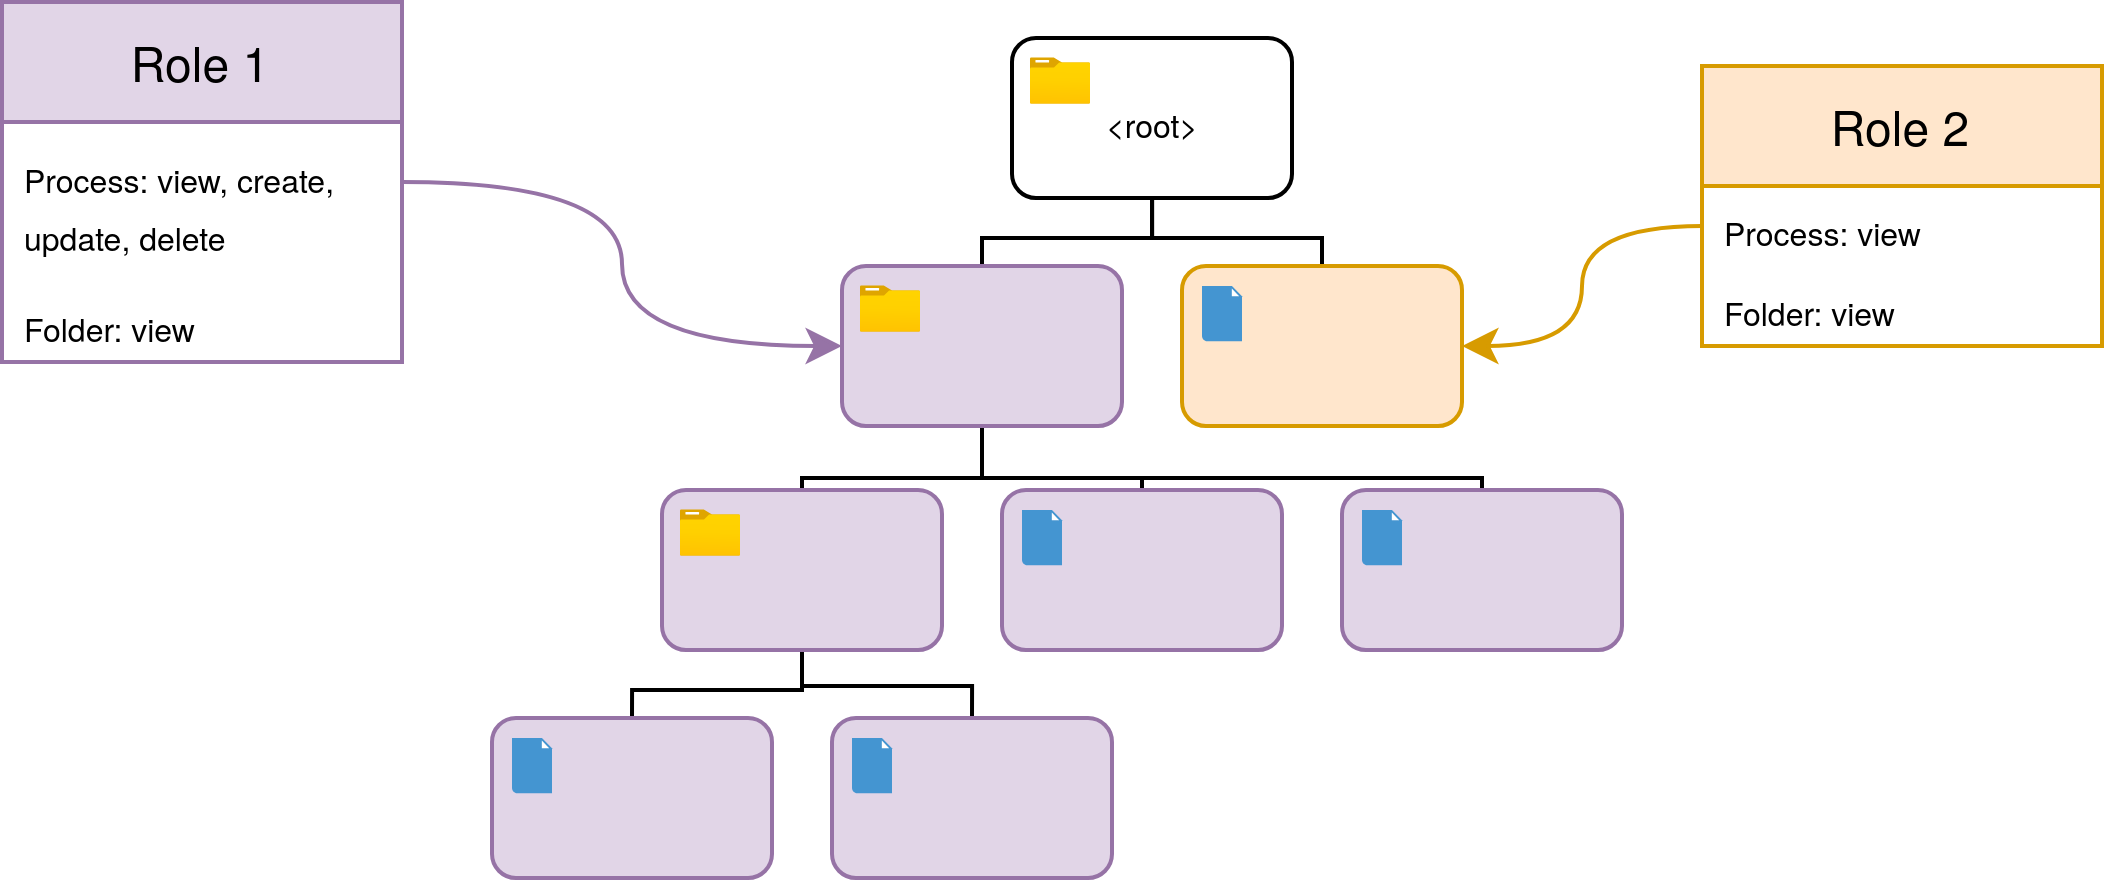
\includegraphics[scale=0.2]{./images/tree-roles.drawio.png}
	\caption{Permissions of roles cascade down the folder structure.}
\end{figure}

If a user's role allows him to view assets and is associated to a folder, then the user
also has the permission to view all ancestors of the folder.
But this permission is only restricted to the parent folders themselves,
not their contents.
This allows users to navigate the folder structure until they reach the assets they're
allowed to view and manage.

% TODOFIG: show how user can view path to his folder

\subsection{New Resources}

% TODO: mention that each role comes with an action
With the introduction of environments, all the previously available resources still hold
the same meaning, with the difference that they are now associated with an environment.
Additionally, two new Resources were introduced, for which roles can specify permissions:

\begin{itemize}
	\item \textbf{Folder}: Folders are used to organize assets in an environment.
	      If a role is associated to a folder, then the permissions for the folder apply to that
	      folder and all folders
	      \begin{itemize}
		      \item \lstinline{view}: Allows the user to view the folder, its name and description.
		            This doesn't necessarily mean that the user can view the assets inside the folder,
		            as he still needs the \lstinline{view} permission for each child.
		      \item \lstinline{create}: The user can create new folders inside the folder he has this
		            permission for.
		      \item \lstinline{update}: The user can update the folder's name and description, as
		            well as move the folder, to another folder where he has the \lstinline{create}
		            permission.

		            % TODO: deleting a folder deletes the processes inside of it
		            % maybe this needs to be checked
		      \item \lstinline[keywords={}]{delete}: The user can delete the folder.
	      \end{itemize}
	\item \textbf{Environment}: Environments are isolated workspaces inside the MS.
    \begin{itemize}
		      % TODO: members cannot actually see the environments name and description 
		      \item \lstinline{view}, \lstinline{create}: These actions are not implemented for
		            environments.
		            Each member can view the name and description of the environment.
		            \lstinline{create} can't exist as it implies that the environment doesn't exist
		            yet, and therefore a role that contains it cannot exist.
		      \item \lstinline{update}: The user can update the environment's name, description
		            and contact number.
            \item \lstinline[keywords={}]{delete}: Allows the user to delete the environment with all its
		            assets, this is only possible for organization environments.
	      \end{itemize}
\end{itemize}

\subsection{Enforcing Permissions Based on the Folder Structure}

In order to enforce permissions based on the folder structure, it is necessary to fetch
the newest state of the folder structure every time a user wants to perform an action on an asset.
Roles can't store a representation of the folder structure, as it might become outdated.
Since permissions need to be verified, for many requests in the MS, and also in the user's browser, to
adapt the UI, we decided to compute and cache a representation of the folder structure of
every organization environment, from which an asset is requested.
This representation is also sent to the user's browser, for the UI to be able to adapt
based on the user's permissions.

% TODO: roles send folder structure to user, is this bad? how could we mitigate it

\subsection{Default Roles}

For each organization environment two roles will be created, which cannot be deleted and
cannot be associated to a folder:

\begin{itemize}
	\item \lstinline{@admin}: This role has all permissions for all assets in the
	      organization environment and it is first assigned to the user that creates the organization environment.
	      Only users with the \lstinline{@admin} role can add new users to this role.
	\item \lstinline{@everyone}: The permissions in this role apply to for all the users
	      that are part of the organization environment. The permissions in this role start out
	      empty, but can be modified.
\end{itemize}

\chapter{Implementation}
\label{cha:implementation}

In this chapter, we will
\footnote{\url{https://github.com/PROCEED-Labs/proceed}}

\section {MS Architecture}
\label{cha:ms-architecture}

Before diving into the implementation details of environments, it is important to
understand the architecture of the MS.
The MS is built using Next.js \footnote{\url{https://nextjs.org/}}, a React \footnote{\url{https://reactjs.org/}}
framework that allows for server-side rendering.
Altough Next.js' architecture is different from traditional server-side rendered
applications and single-page applications,
for the purposes of this thesis,
it can be thought of as being split into a single-page frontend and a backend.
The frontend executes JavaScript code in the user's browser, and is
responsible for rendering the UI, handling user input and making requests to the backend.
The backend runs on a server and is responsible for handling requests from the frontend,
e.g. saving or querying data.

\subsection{Data storage}
\label{cha:ms-architecture:data-storage}

% TODO: footnote or something for json

The MS doesn't use a database management system, instead it stores all data in JSON files.
Each file can be seen as a table in a traditional relational database.
Even though this approach allows for unstructured data, the MS uses 
Zod \footnote{\url{https://zod.dev/}} schemas to enforce a structure on
data that is stored.
Zod is a schema declaration and validation library, it allows the MS to define the shape
of JSON serializable data.
For purposes of simplicity, when we talk about a schema, instead of showing the code that
describes the Schema, we will show the typescript type that satisfies the schema.

\begin{lstlisting}[
  language=JavaScript,
  style=codestyle,
  caption={Example of a Zod schema and the corresponding TypeScript type.},
]
import { z } from 'zod';

const UserSchema = z.object({
  id: z.string(),
  username: z.string(),
  image: z.string().optional(),
})

// TypeScript type that satisfies the UserSchema
type User = {
    id: string;
    username: string;
    image?: string | undefined;
}
\end{lstlisting}

% TODO: either finish this or remove it
% Additionally, the MS stores XML files for BPMN Assets.

\section{Users}


%
% \begin{lstlisting}[
%   language=JavaScript,
%   style=codestyle,
%   caption={Example setup of NextAuth.js.},
% ]
% const handler = NextAuth(nextAuthOptions);
% \end{lstlisting}

% TODO: this section
\subsection{Sign in flows}

User authentication is implemented by leveraging OpenID Connect\ref{cha:relatedwork:oauth:openid},
with the help of NextAuth.js\footnote{\url{https://next-auth.js.org/}}.
A JWT token \footnote{\url{https://www.rfc-editor.org/rfc/rfc7519.txt}}
is stored in the user's browser cookies\footnote{\url{https://www.rfc-editor.org/rfc/rfc7519.html}},
which is then parsed and verified by the MS' backend.
% TODO: is "id" the correct word here
If the JWT token is valid the user is considered authenticated.
If the user couldn't be authenticated, he is redirected to the sign-in page.

NextAuth.js has many sign-in methods built-in, which can be set up with little configuration.
For email-sign in, NextAuth.js sends an email with a link that the user has to click to
sign in.
We have to provide a way to store and query the tokens, that are encoded in the link and a
function that sends the email.
For OAuth2 providers, we only have to provide a client id and secret.

To store and look up users and accounts, NextAuth.js requires a database adapter,
which is a set of functions that interact with the database.
% TODO: add ref
The structure of the data that will be stored described in \ref{}.

NextAuth.js provides hooks that allow us to customize the sign-in flow, the most important
one for this thesis is the \lstinline{signIn} hook.
This hook is called when a user tries to sign in, this can be a new user or a returning
one.
As arguments, it receives the user's data, and the account that the user is trying to sign
in, if the user doesn't exist the user data may be empty.
If the hook returns true, the sign-in flow continues, if it returns a string or false,
then the sign-in flow is stopped, and the user is redirected to an error page.
Inside this hook, we can also check if the user was previously signed-in as a guest user
and is now signing in with personal information, so that we can merge the data of the two,
we will elaborate on this in \ref{cha:ms-architecture:merge-guest-user-data}.

% TODO: decicde if we need a setup example for nextauth.js

\begin{lstlisting}[
  language=JavaScript,
  style=codestyle,
  caption={Schema for authenticated users.},
]
import NextAuth from 'next-auth/next';
import GoogleProvider from 'next-auth/providers/google';

const authOptions = {
  providers: [
    EmailProvider({
      sendVerificationRequest({ url }) {
        // send email
      },
    }),
    GoogleProvider({
      clientId: process.env.GOOGLE_CLIENT_ID,
      clientSecret: process.env.GOOGLE_CLIENT_SECRET,
    }),
  ],
}

const handler = NextAuth(authOptions)
\end{lstlisting}


% (property) signIn?: ((params: {
%     user: User | AdapterUser;
%     account: Account | null;
%     profile?: Profile | undefined;
%     email?: {
%         verificationRequest?: boolean | undefined;
%     } | undefined;
%     credentials?: Record<string, CredentialInput> | undefined;
% }) => Awaitable<string | boolean>) | undefined
%
% Use this callback to control if a user is allowed to sign in.
% Returning true will continue the sign-in flow.
% Throwing an error or returning a string will stop the flow, and redirect the user.
%
% [Documentation](https://next-auth.js.org/configuration/callbacks#sign-in-callback)


\subsection{Authenticated Users}
\label{cha:ms-architecture:authenticated-users}

Authenticated Users are users that sign in to the MS either with their email or with a
OAuth 2.0 provider.
They're stored in the MS by NextAuth.js after they've successfully signed in.
For authenticated users we store an \lstinline{id}, a flag named \lstinline{isGuest}, set
to false, and personal information. 
This is the schema for authenticated users:

% NOTE: maybe explain that because of nextauths weirdness the email is just stored in the
% user instead of the account

\begin{lstlisting}[
  language=JavaScript,
  style=codestyle,
  caption={Schema for authenticated users.},
  label={lst:authenticated-users-schema}
]
{
    id: string;
    isGuest: false;
    emailVerifiedOn: Date | undefined;
    firstName?: string | undefined;
    lastName?: string | undefined;
    username?: string | undefined;
    image?: string |  undefined;
    email?: string | undefined;
}

\end{lstlisting}

All the personal information is optional, because depending on how the user signs in, the
information might not be available.
For instance, because NextAuth.js' email sign in only requires the user to input an
email, authenticated users are created without a first name, last name or username.
A possible workaround would be to automatically generate these, but we chose to leave them
undefined, and prompt the user to fill them when he first signs in.


\begin{figure}[H]
    \centering
    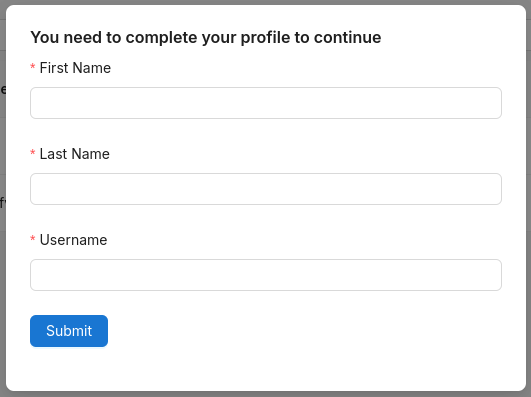
\includegraphics[scale=0.4]{images/fill-data-prompt.png}
    \caption{Prompt to fill in personal information.}
    \vspace{-1em} % Negative value to remove space
    \label{fig:prompt-fill-personal-information}
\end{figure}

% TODO: cite paper or something to show that this can happen?? im sure theres going to be
% smth
The \lstinline{image} field is used to store a URL to a user's profile picture. This field
can only be set if the user signed in with an OAuth 2.0, which supplied
the URL.
We don't accept custom URLs, as this allows for attackers to supply URLs to a server he
controls, which can be used to track user's browsers.
By only saving URLs provided directly by trusted OAuth 2.0 providers, we ensure that the
source of the image is reliable.

As stated before, we need Accounts, to store the sign-in methods of a user.
To recognize a user's account we need to store the name of the provider and the account's.
ID on the provider's platform.
Additionally, to link the account to a user, we store the user's ID in the account.
The schema for accounts is as follows:

\begin{lstlisting}[
  language=JavaScript,
  style=codestyle,
  caption={Schema for accounts.},
]
{
    id: string;
    type: "oauth";
    userId: string;
    provider: string;
    providerAccountId: string;
}
\end{lstlisting}

\subsection{Guest Users}

Users that aren't signed in can choose to try the MS out as a guest, this doesn't require
the user to input any personal information.
For users that choose to sign in as a guest, a new user is created and stored in the MS.
To achieve this, we use a modified version of the authenticated user schema described in
\ref{lst:authenticated-users-schema}, to only include the \lstinline{id} and the
\lstinline{isGuest} flag set to true.

\begin{lstlisting}[
  language=JavaScript,
  style=codestyle,
  caption={Schema for guest users.},
]
{
    isGuest: true;
    id: string;
} 
\end{lstlisting}

This option must be made available to users during the sign-in process. 
To accomplish this, NextAuth.js provides a built-in \lstinline{CredentialsProvider}, 
which enables the implementation of custom sign-in methods. 
We configured this provider to accept no credentials,
allowing users to sign in without supplying personal information.

\begin{lstlisting}[
  language=JavaScript,
  style=codestyle,
  caption={Custom sign-in method for guest users.},
]
import NextAuth from 'next-auth/next';

const authOptions = {
  providers: [
    ...
    CredentialsProvider({
      name: 'Continue as Guest',
      credentials: {},
      async authorize() {
        return addUser({ isGuest: true });
      },
    }),
  ],
}

const handler = NextAuth(authOptions)
\end{lstlisting}

After a user signs in as a guest, a JWT token is stored in his cookies.
Since there is no personal information stored, there is no way for the user to sign in to
his guest account from another device.
This also means, that if the cookies are deleted, the user will lose access to his guest account.

\subsection{Merge guest user data with an authenticated user's data}
\label{cha:ms-architecture:merge-guest-user-data}

When a guest user decides to sign in with personal information, we have to merge the data

\subsection{Development users}
\label{cha:ms-architecture:users:development-users}

\section{Assets}

- environmentId stored on each thing to improve querying
- talk about data normalization
- talk about breaking normalization for perfomance gains -> reference a paper or smth

\section{Environments}

- environments are entry in db
- memberships
- environment format entry
- verification (when envs are created by not signed in users)
- creation
- deletion - managing the env
- section for folders
- decide how to divide 

Environments are stored as an entry in the MS table


\subsection{Creation}
\subsection{Memberships}

\section{Roles}





In this chapter we will evaluate the implementation of environments in the PROCEED MS,
for this we will go through the requirements defined in \ref{cha:tasklist}.
The primary goals of this thesis were to introduce environments as isolated workspaces for personal and organizational use,
enable efficient asset management through a hierarchical folder structure,
and adapt the MS's a role-based access control system to fit environments.
The following \ref{fig:quick-evaluation} table shows a quick rundown of the evaluation.


\begin{figure}[H]
	\centering

	\begin{tabular}{ | m{20em} | m{17em}| }
		\hline
		 Task & Status \\
     \hline
      1. Implement environments &  Partially implemented: folders were only implemented for processes. \\
     \hline
      2. Personal and organization Environments &  Implemented \\
     \hline
      3. Adapt the MS' user management system to fit environments &  Implemented \\
     \hline
      4. Adapt the MS' role system to fit environments &  Implemented \\
     \hline
  %    1.a & x \\
		%  1.b &  \\
		%  1.c &  \\
		%  1.d &  \\
		%
		%  2.a &  \\
		%  2.b &  \\
		%  2.c &  \\
		%  2.d &  \\
		%  2.e &  \\
		%  2.f &  \\
		%  2.g &  \\
		%  3.a & \\
		%
		%  3.b.i &  \\
		%
		%  3.b.ii &  \\
		%  3.b.iii &  \\
		%  3.b.iv &  \\
		%  3.c &  \\
		%  3.d &  \\
		%
		%  4.a &  \\
		%  4.b &  \\
		%  4.c &  \\
		%  4.d &  \\
		%  4.e &  \\
		% ------------------------------------------------------------------------------
	\end{tabular}

	\caption{Evaluation of Task List.}
	\label{fig:quick-evaluation}
\end{figure}

According to \textbf{task 1} Environments are stored as entries in the MS's storage
solution with a unique id.
Every asset in the MS explicitly stores the id of the environment it belongs to.
Memberships to environments are stored in a separate table, where each entry has a user id
and an environment id,
later on we will explain how the access to assets is managed.
Furthermore, each environment has a root folder, which contains more folders and
processes.
Apart from root folders, both process and folders store the id of the folder they belong
to.

According to \textbf{task 2} environments store a flag to determine whether they are a
personal or an organization environment.
Personal environments are created when a user is created and organization environments can
be created by signed-in users.
Personal environments have a restricted feature-set, this is enforced by the role
system, this will be explained in more detail when we address task 4.
Users in organization environments can potentially use all the MS's features, this is
determined by the roles they have inside that environment.
The user that creates an organization environment is assigned the role of admin inside
that environment.
Access to assets in organization environments is managed by the role system described in
task 4,
the admin role has all permissions for all assets in the environment.
Organization environments can have multiple members, new members can be invited by other
members with the right permissions.

According to \textbf{task 3}, the user management was redesigned to accommodate
multi-tenancy,
users are now stored as records in the MS's storage solution independently of the environments they belong to.
This allows for them to be part of multiple environments.
Users also have the option to sign in as a guest, which allows them to try the MS inside
a personal environment without having to sign up.
Guest users are stored as other users, but with a flag that indicates that they are a
guest.

According to \textbf{task 4}, the MS's role system was adapted to fit environments and
folders. In its essence, roles work as they do before with two key differences:
Each role belongs to an environment and is only applied for assets inside that
environment, and roles can be scoped to folders, meaning that its permissions apply on all
descendants of the folder.
The role system was also leveraged to restrict the feature set of personal environments:
while personal environments don't have roles, the MS still uses the role system to manage
access to assets inside personal environments, it gives the owner of the environment all
permissions for the allowed features and restricts the rest.

\ref{cha:tasklist} also describes a set of non-functional requirements, these are harder
to evaluate than functional requirements. For these reason we surveyed other developers
that are working on the MS to get their opinion on the implementation of environments. 
The following questions were asked:



\chapter{Conclusion}
\label{cha:conclusion}

Building an application structure that supports multi-tenancy presents many challenges,

This thesis addressed the challenge of implementing multi-tenancy in the PROCEED
Management System (MS).

by introducing the concept of environments. These environments
offer isolated workspaces for users, supporting both personal and organizational use cases
while maintaining the flexibility and security required for cloud-based applications.


The shift to multi-tenancy required rethinking how assets and users are stored. 
We introduced personal environments, where a single user can manage assets privately, and
organization environments, where multiple users can collaborate on shared folders and
processes. 
Along with the environment concept, we adapted the existing role system so that
permissions now respect both the folder hierarchy and environment boundaries, ensuring
that users only interact with assets they are supposed to.

A major focus was to keep the underlying code changes minimal and 
to make the new abstraction straightforward to use from a developer perspective.
Enforcing access rules in the backend through CASL and providing helper functions for the
frontend were crucial steps to maintain security and consistency across the MS.
We also paid careful attention to the handling of guest users, giving them the option to merge
their data with fully authenticated accounts without losing the assets they created.

Overall, the work presented here lays the foundation for a robust multi-tenant experience in the PROCEED MS. It strikes a balance between introducing an entirely new concept—environments—and preserving the existing structure of the system so that both end users and developers can comfortably adapt to the new features.







\section{Outlook}
\label{cha:outlook}

Nowadays software is so advanced in multi tenant platforms, companies have come to expect
a lot of features from such software.
Other than the role system this thesis implements the bare minimum to provide such an
experience.
There are still many features that could be implemented to improve the expierience.

- sharing documents to members that arent part of the organization
- Support for user directives -> everyone doesn't have to create an account manually
  - here it could be also possible that an organization is created and all accounts from
    the user directive are automatically added 
-


%--------------------------------------------------------------
% TABLES, FIGURES, BIBLOGRAPHY AND APPENDICES
%--------------------------------------------------------------
\backmatter

% Lists of tables and figures
\listoftables
\listoffigures

% Bibliography
\setwidesite{}						% Set page to be wider for bibliography
\markboth{Bibliography}{bibliography}
\label{cha:bibliography}
\bibliographystyle{IEEEtran}
\bibliography{bibliography.bib}

% Use following to separate online (websites) and offline (books, papers) sources
%\printbibliography[heading=offline,filter=offline]
%\printbibliography[heading=online,filter=online]

\begin{appendices}
	% \chapter{Appendix 1}
% \label{appendix:listing1}
%
% \lstset{language=PHP}
% \begin{lstlisting}
% for($i=1; $i<123; $i++)
% {
%     echo "work harder! ;)";
% }
% \end{lstlisting}

	% \input{content/99_appendices/a02_listings}
	% \input{content/99_appendices/a03_listings}
\end{appendices}

\end{document}
